% Ensure that you compile using XeLaTeX !!! PDFTex has problems with some of the packages used
\documentclass[12pt]{article}
\setlength\parindent{0pt}

\usepackage{parskip}
\usepackage[margin=0.5in]{geometry}
\usepackage{fullpage}
\usepackage{moresize}
\usepackage{graphicx}
\usepackage{caption}
\usepackage{subcaption}
\usepackage{float}
\usepackage{xcolor}
\usepackage{soul}
\usepackage{fontspec}
\setmainfont{Doulos SIL}

\begin{document}

\begin{center}
\textbf{{\color{violet}{\HUGE Friday, 5 June 2020\\}}}

\textbf{{\color{violet}{\HUGE ALL EXAMS\\}}}

\end{center}
\newpage

\begin{center}
\textbf{{\color{blue}{\HUGE START OF EXAM\\}}}

\textbf{{\color{blue}{\HUGE Student ID: 6745\\}}}

\textbf{{\color{blue}{\HUGE 11:30 - 11:45 AM\\}}}

\end{center}
\newpage

{\large Question 1}\\

Source: Quiz 3, Question 2\\

L$_X$ has tri-syllabic roots. If L$_X$ does not allow non-identical high vowels to co-occur, which one of the following tri-syllabic vocalic sequences do you predict to be unattested in L$_X$? Explain why.\\

\begin{itemize} \item {[u...i...a]} \item {[a...i...a]} \item {[u...u...a]} \item {[a...i...i]} \end{itemize}


\newpage

{\large Question 2}\\

Source: Day 4 Handout, Question 3\\

Explain how you would figure out what the Luiseño form is for the morpheme whose meaning is given below.\\

‘walk’

\begin{figure}[H]
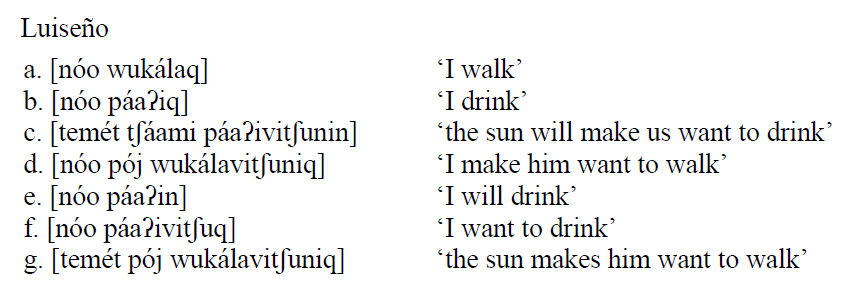
\includegraphics{../images/luiseno.png}
\end{figure}

\newpage

{\large Question 3}\\

Source: Day 6 Handout, Question 11\\

What do the two signs below tell you about the phonological status of \underline{handshape} in ASL, and why?\\

\begin{figure}[H]
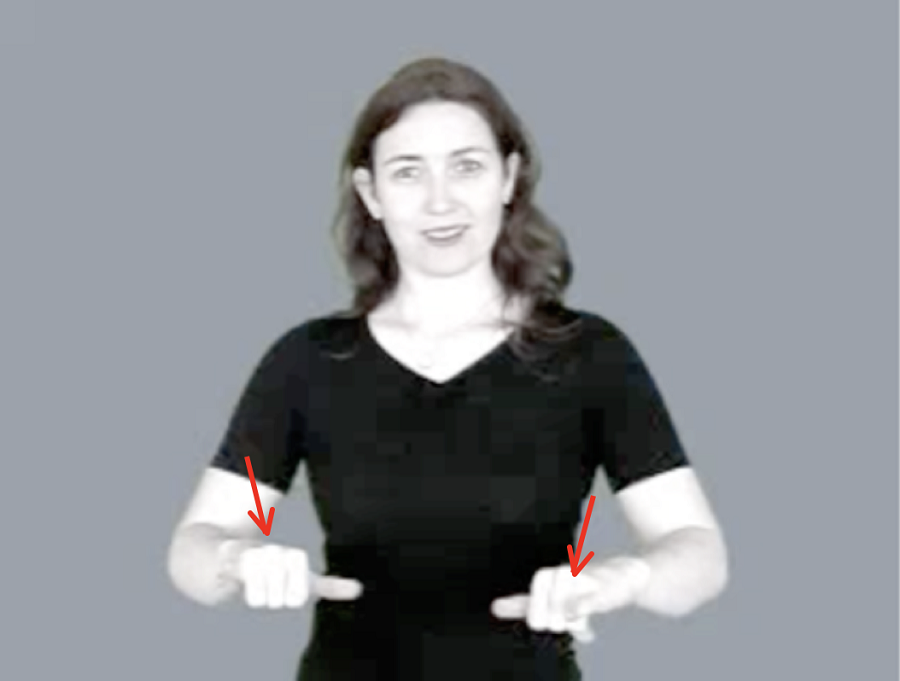
\includegraphics{../images/asl_stay.png}
\caption{STAY}
\end{figure}
\begin{figure}[H]
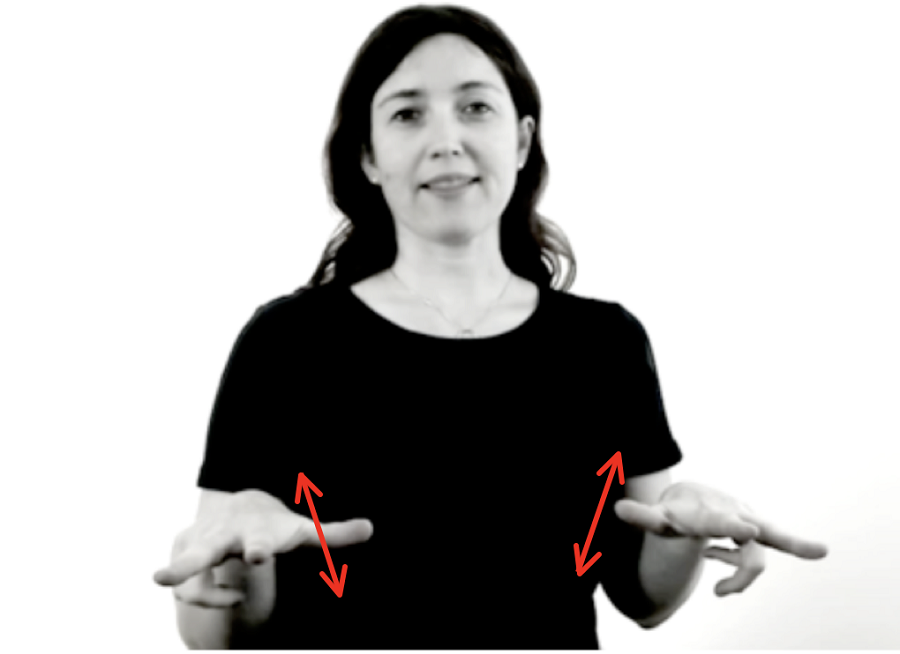
\includegraphics{../images/asl_awkward.png}
\caption{AWKWARD}
\end{figure}

\newpage

{\large Question 4}\\

Source: Homework 1, Question 3(b)\\

Explain why this is or is not a complete natural class in standard North American English.\\

{[i]}, {[u]}, {[eɪ]}


\newpage

{\large Question 5}\\

Source: Day 2 Handout, Part I, Question 11\\

How would this word be transcribed?\\ Follow-up question: Why did you use symbol [X] instead of symbol [Y]?\\

<goat>


\newpage

\begin{center}
\textbf{{\color{red}{\HUGE END OF EXAM}}}\\

\end{center}
\newpage

\begin{center}
\textbf{{\color{blue}{\HUGE START OF EXAM\\}}}

\textbf{{\color{blue}{\HUGE Student ID: 9303\\}}}

\textbf{{\color{blue}{\HUGE 11:45 AM - 12:00 noon\\}}}

\end{center}
\newpage

{\large Question 1}\\

Source: Quiz 3, Question 2\\

L$_X$ has tri-syllabic roots. If L$_X$ does not allow non-identical high vowels to co-occur, which one of the following tri-syllabic vocalic sequences do you predict to be unattested in L$_X$? Explain why.\\

\begin{itemize} \item {[u...i...a]} \item {[a...i...a]} \item {[u...u...a]} \item {[a...i...i]} \end{itemize}


\newpage

{\large Question 2}\\

Source: Day 2 Handout, Part II, Question 9\\

Explain how to figure out what the sound being produced is in this diagram.\\

\begin{figure}[H]
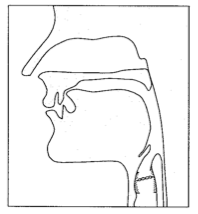
\includegraphics{../images/sagittal_z.png}
\end{figure}

\newpage

{\large Question 3}\\

Source: Day 6 Handout, Question 11\\

What do the two signs below tell you about the phonological status of \underline{handshape} in ASL, and why?\\

\begin{figure}[H]
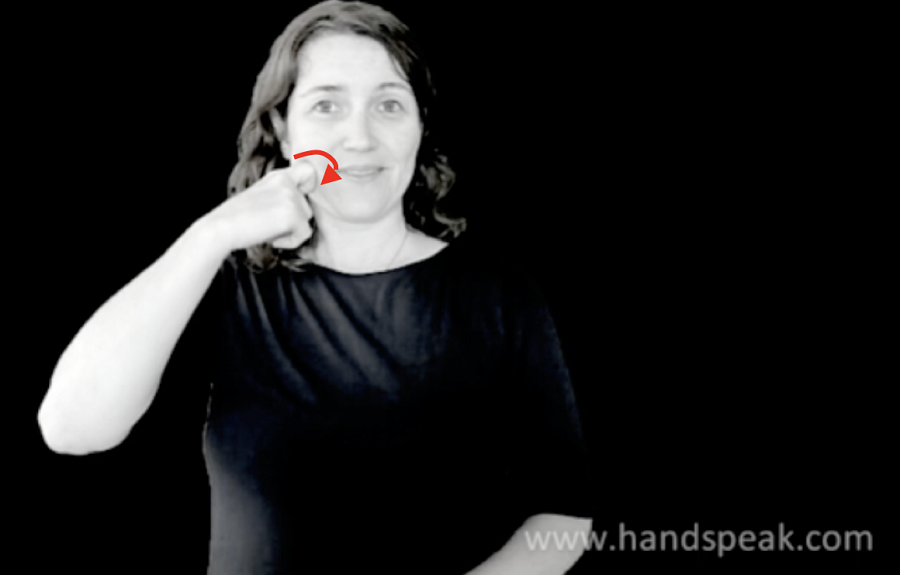
\includegraphics{../images/asl_apple.png}
\caption{APPLE}
\end{figure}
\begin{figure}[H]
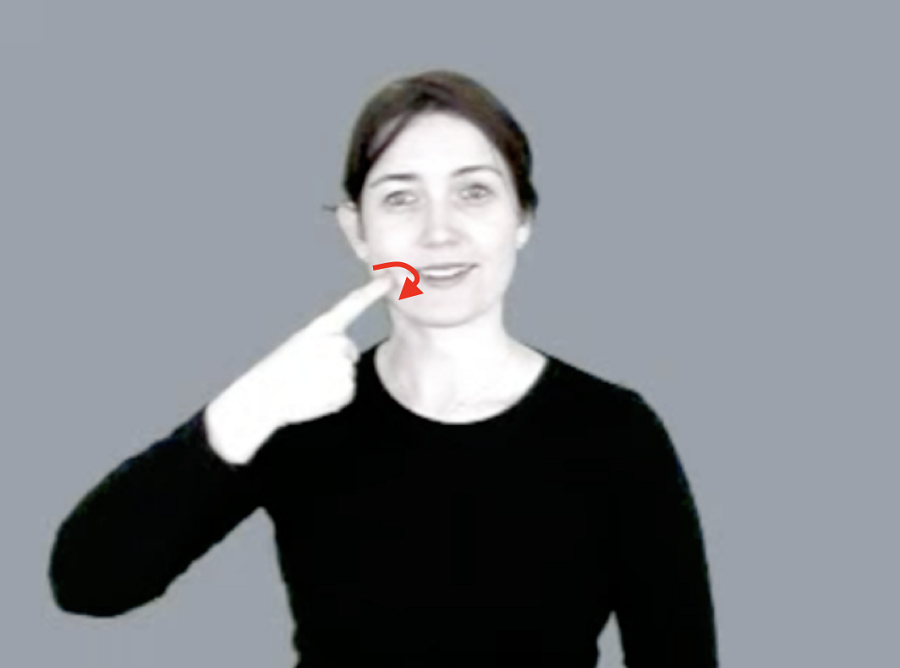
\includegraphics{../images/asl_candy.png}
\caption{CANDY}
\end{figure}

\newpage

{\large Question 4}\\

Source: Day 2 Handout, Part I, Question 11\\

How would this word be transcribed?\\ Follow-up question: Why did you use symbol [X] instead of symbol [Y]?\\

<square>


\newpage

{\large Question 5}\\

Source: Day 2 Handout, Part I, Question 11\\

How would this word be transcribed?\\ Follow-up question: Why did you use symbol [X] instead of symbol [Y]?\\

<toy>


\newpage

\begin{center}
\textbf{{\color{red}{\HUGE END OF EXAM}}}\\

\end{center}
\newpage

\begin{center}
\textbf{{\color{blue}{\HUGE START OF EXAM\\}}}

\textbf{{\color{blue}{\HUGE Student ID: 8079\\}}}

\textbf{{\color{blue}{\HUGE 12:00 noon - 12:15 PM\\}}}

\end{center}
\newpage

{\large Question 1}\\

Source: Quiz 3, Question 1\\

L$_X$ (Language X) has three vowels, [i], [a], and [u]. It has bi-syllabic roots like Kikuyu. It does not allow non-identical high vowels to co-occur. Of the following nine logically possible vocalic sequences, which ones should be unattested in L$_X$? Explain why.\\

\begin{itemize} \item {[i...i]} \item {[i...a]} \item {[i...u]} \item {[a...i]} \item {[a...a]} \item {[a...u]} \item {[u...i]} \item {[u...a]} \item {[u...u]} \end{itemize}


\newpage

{\large Question 2}\\

Source: Day 2 Handout, Part I, Question 11\\

How would this word be transcribed?\\ Follow-up question: Why did you use symbol [X] instead of symbol [Y]?\\

<vacuum>


\newpage

{\large Question 3}\\

Source: Homework 1, Question 3(b)\\

Explain why this is or is not a complete natural class in standard North American English.\\

{[j]}, {[w]}


\newpage

{\large Question 4}\\

Source: Day 2 Discussion\\

Assuming a Standard North American English inventory, does this vowel need to have tenseness specified if you're giving a prose description? Why or why not?\\

{[i]}


\newpage

{\large Question 5}\\

Source: Day 7 Handout, Question 9\\

What is the basic analysis of vowel length in this dataset, and what are the key pieces of evidence?\\

\begin{figure}[H]
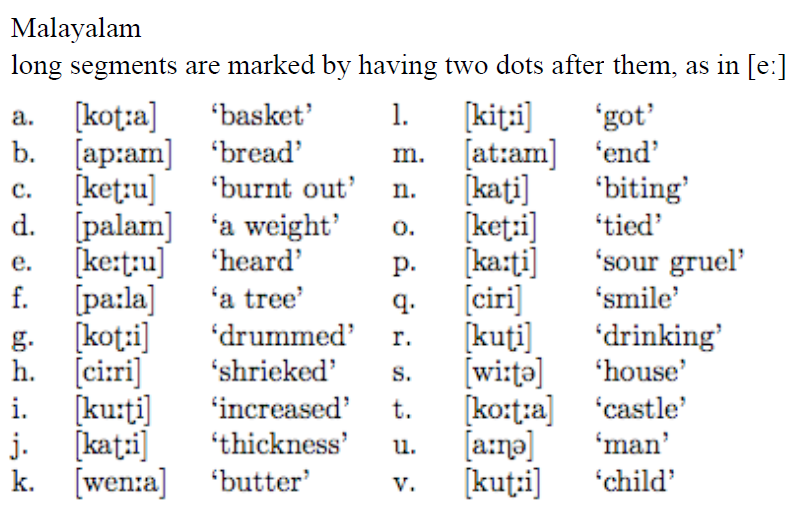
\includegraphics{../images/malayalam.png}
\end{figure}

\newpage

\begin{center}
\textbf{{\color{red}{\HUGE END OF EXAM}}}\\

\end{center}
\newpage

\begin{center}
\textbf{{\color{blue}{\HUGE START OF EXAM\\}}}

\textbf{{\color{blue}{\HUGE Student ID: 1794\\}}}

\textbf{{\color{blue}{\HUGE 12:15 PM - 12:30 PM\\}}}

\end{center}
\newpage

{\large Question 1}\\

Source: Quiz 3, Question 2\\

L$_X$ has tri-syllabic roots. If L$_X$ does not allow non-identical high vowels to co-occur, which one of the following tri-syllabic vocalic sequences do you predict to be unattested in L$_X$? Explain why.\\

\begin{itemize} \item {[u...i...a]} \item {[a...i...a]} \item {[u...u...a]} \item {[a...i...i]} \end{itemize}


\newpage

{\large Question 2}\\

Source: Day 2 Handout, Part I, Question 11\\

How would this word be transcribed?\\ Follow-up question: Why did you use symbol [X] instead of symbol [Y]?\\

<segment>


\newpage

{\large Question 3}\\

Source: Day 7 Handout, Question 12\\

What is the basic analysis of oral and nasal vowels in this dataset, and what are the key pieces of evidence?\\

\begin{figure}[H]
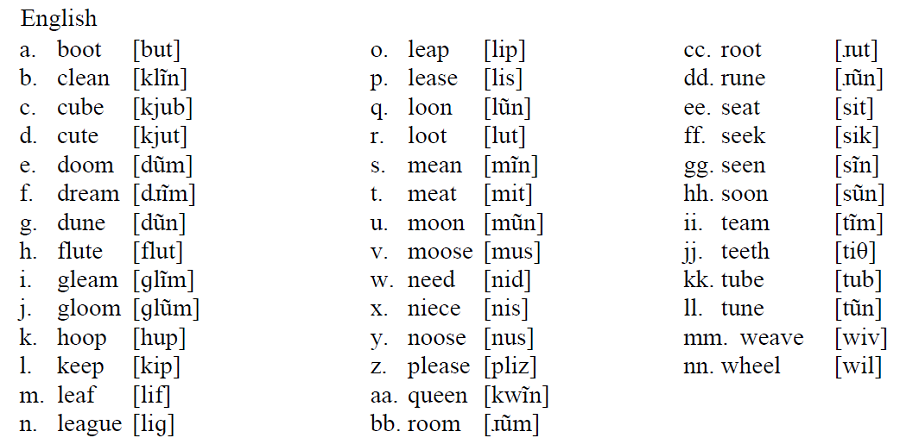
\includegraphics{../images/english12.png}
\end{figure}

\newpage

{\large Question 4}\\

Source: Day 2 Handout, Part I, Question 11\\

How would this word be transcribed?\\ Follow-up question: Why did you use symbol [X] instead of symbol [Y]?\\

<nice>


\newpage

{\large Question 5}\\

Source: Homework 1, Question 3(b)\\

Explain why this is or is not a complete natural class in standard North American English.\\

{[j]}, {[w]}


\newpage

\begin{center}
\textbf{{\color{red}{\HUGE END OF EXAM}}}\\

\end{center}
\newpage

\begin{center}
\textbf{{\color{blue}{\HUGE START OF EXAM\\}}}

\textbf{{\color{blue}{\HUGE Student ID: 2357\\}}}

\textbf{{\color{blue}{\HUGE 12:30 - 12:45 PM\\}}}

\end{center}
\newpage

{\large Question 1}\\

Source: Day 5 Handout, Question 5\\

How would you look for co-occurrence restrictions between [s] and the vowels that come after it in this dataset?\\

\begin{figure}[H]
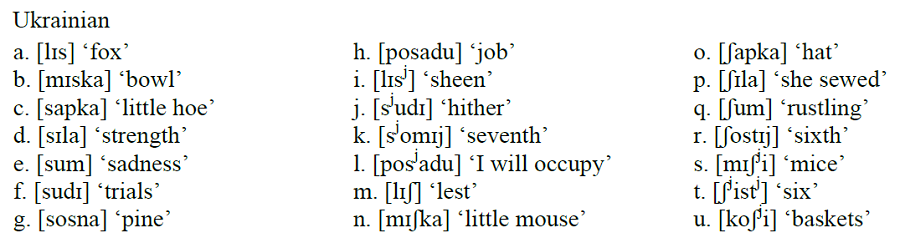
\includegraphics{../images/ukrainian.png}
\end{figure}

\newpage

{\large Question 2}\\

Source: Day 4 Handout, Question 2(iii)\\

Explain how you would figure out the meaning of this Swahili word.\\

{[umefika]}

\begin{figure}[H]
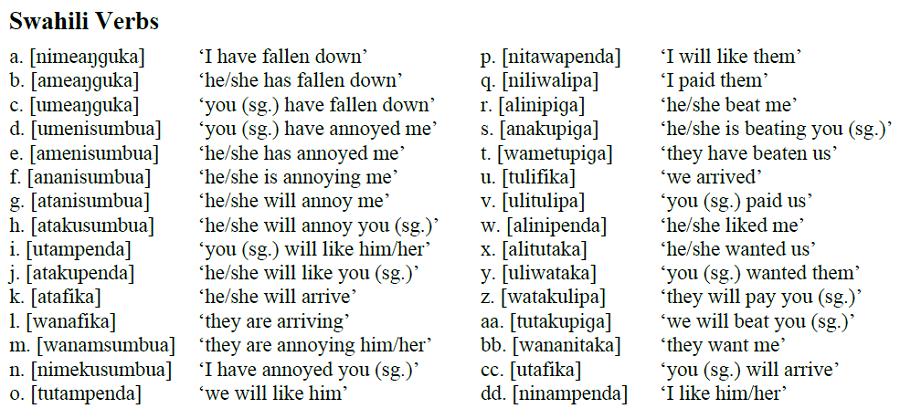
\includegraphics{../images/swahiliverbs.png}
\end{figure}

\newpage

{\large Question 3}\\

Source: Day 2 Handout, Part I, Question 11\\

How would this word be transcribed?\\ Follow-up question: Why did you use symbol [X] instead of symbol [Y]?\\

<goat>


\newpage

{\large Question 4}\\

Source: Day 2 Handout, Part II, Question 9\\

Explain how to figure out what the sound being produced is in this diagram.\\

\begin{figure}[H]
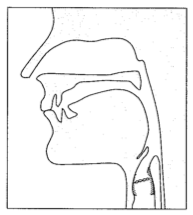
\includegraphics{../images/sagittal_m.png}
\end{figure}

\newpage

{\large Question 5}\\

Source: Day 6 Handout, Question 11\\

What do the two signs below tell you about the phonological status of \underline{handshape} in ASL, and why?\\

\begin{figure}[H]
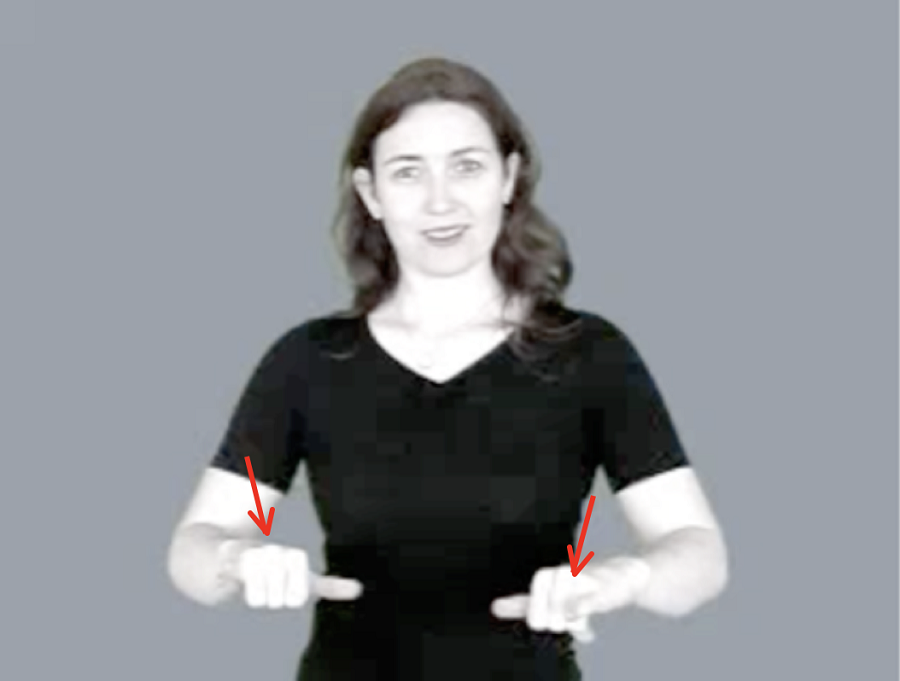
\includegraphics{../images/asl_stay.png}
\caption{STAY}
\end{figure}
\begin{figure}[H]
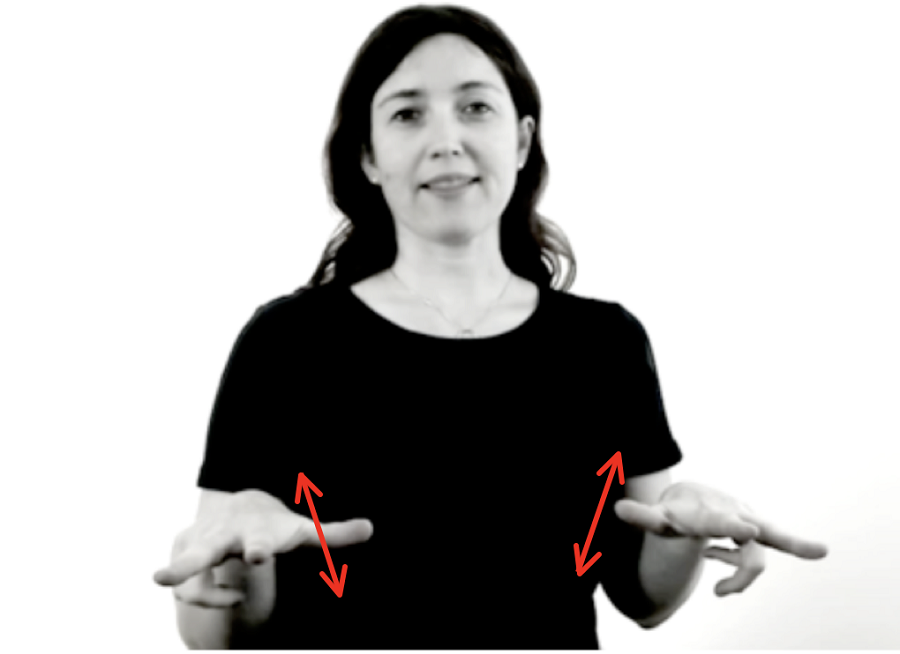
\includegraphics{../images/asl_awkward.png}
\caption{AWKWARD}
\end{figure}

\newpage

\begin{center}
\textbf{{\color{red}{\HUGE END OF EXAM}}}\\

\end{center}
\newpage

\begin{center}
\textbf{{\color{blue}{\HUGE START OF EXAM\\}}}

\textbf{{\color{blue}{\HUGE Student ID: 3773\\}}}

\textbf{{\color{blue}{\HUGE 12:45 - 1:00 PM\\}}}

\end{center}
\newpage

{\large Question 1}\\

Source: Quiz 3, Question 2\\

L$_X$ has tri-syllabic roots. If L$_X$ does not allow non-identical high vowels to co-occur, which one of the following tri-syllabic vocalic sequences do you predict to be unattested in L$_X$? Explain why.\\

\begin{itemize} \item {[u...i...a]} \item {[a...i...a]} \item {[u...u...a]} \item {[a...i...i]} \end{itemize}


\newpage

{\large Question 2}\\

Source: Day 2 Handout, Part II, Question 7\\

Is the symbol given a reasonable way to transcribe any of the sounds described below? If so, which one? If not, why not?\\

{[θ]}

\begin{itemize} \item voiceless palatal affricate \item voiced velar nasal \item voiceless glottal fricative \item voiced labiodental fricative \item voiced interdental fricative \item voiced palatal fricative \end{itemize}


\newpage

{\large Question 3}\\

Source: Day 6 Handout, Question 11\\

What do the two signs below tell you about the phonological status of \underline{handshape} in ASL, and why?\\

\begin{figure}[H]
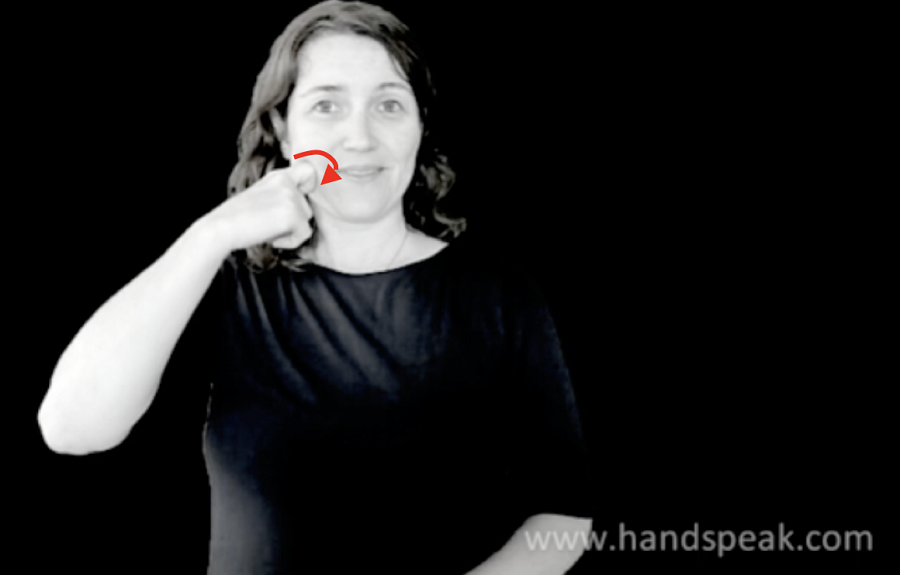
\includegraphics{../images/asl_apple.png}
\caption{APPLE}
\end{figure}
\begin{figure}[H]
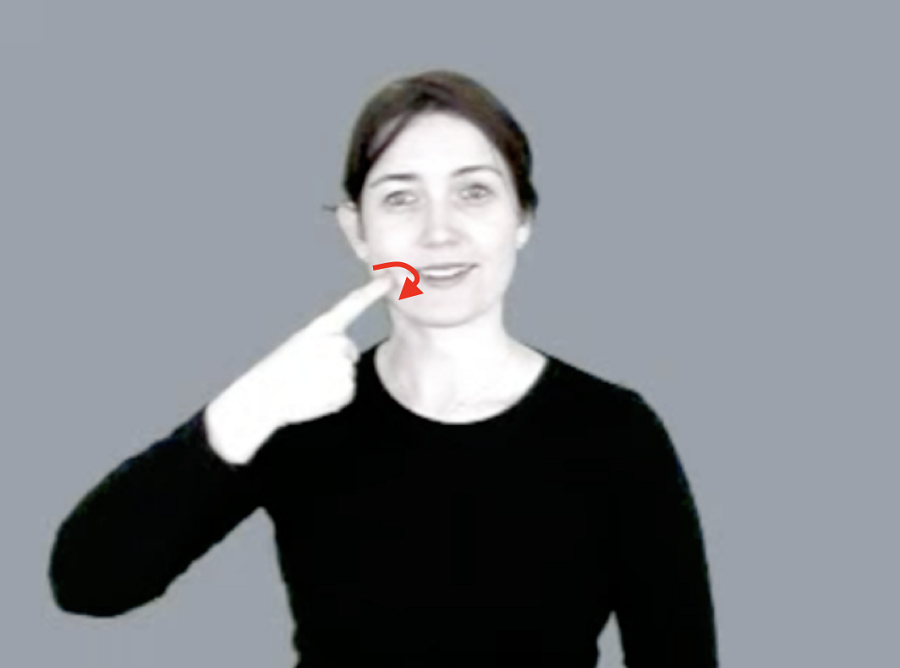
\includegraphics{../images/asl_candy.png}
\caption{CANDY}
\end{figure}

\newpage

{\large Question 4}\\

Source: Day 2 Handout, Part I, Question 11\\

How would this word be transcribed?\\ Follow-up question: Why did you use symbol [X] instead of symbol [Y]?\\

<vacuum>


\newpage

{\large Question 5}\\

Source: Day 7 Handout, Question 2\\

Explain whether the rule below would apply to the form shown, and if so, what the effect of the rule would be. Assume the vowel inventory [i], [ɪ], [e], [ɛ], [ɑ], [u], [ʊ], [o], [ɔ].\\

/emus/

{[high vowel]} →  {[unround, front]} / {[front vowel]} C$_0$ \_\_ 


\newpage

\begin{center}
\textbf{{\color{red}{\HUGE END OF EXAM}}}\\

\end{center}
\newpage

\begin{center}
\textbf{{\color{blue}{\HUGE START OF EXAM\\}}}

\textbf{{\color{blue}{\HUGE Student ID: 8951\\}}}

\textbf{{\color{blue}{\HUGE 1:00 - 1:15 PM\\}}}

\end{center}
\newpage

{\large Question 1}\\

Source: Day 5 Handout, Question 5\\

How would you look for co-occurrence restrictions between [s] and the vowels that come after it in this dataset?\\

\begin{figure}[H]
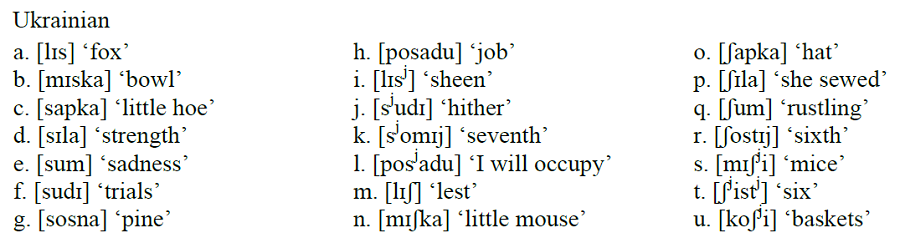
\includegraphics{../images/ukrainian.png}
\end{figure}

\newpage

{\large Question 2}\\

Source: Day 6 Handout, Question 11\\

What do the two signs below tell you about the phonological status of \underline{handshape} in ASL, and why?\\

\begin{figure}[H]
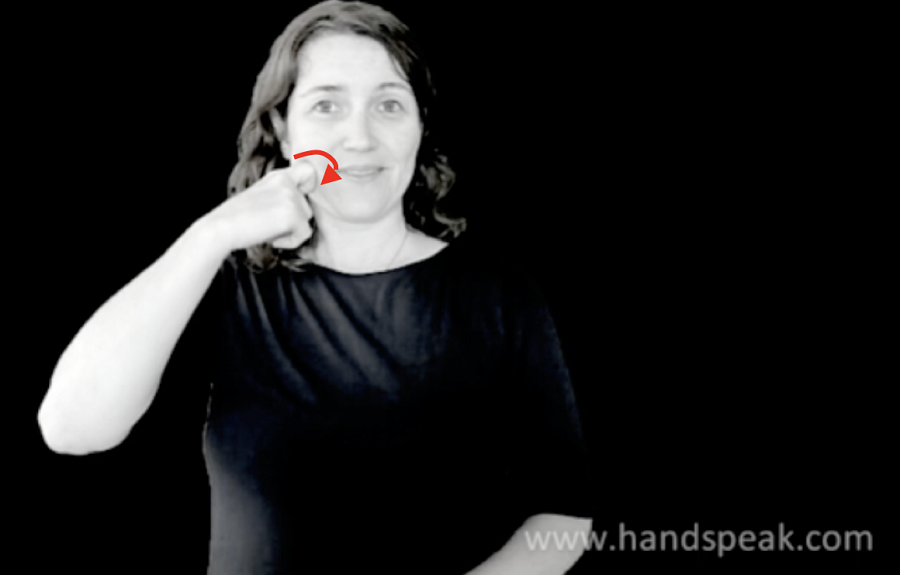
\includegraphics{../images/asl_apple.png}
\caption{APPLE}
\end{figure}
\begin{figure}[H]
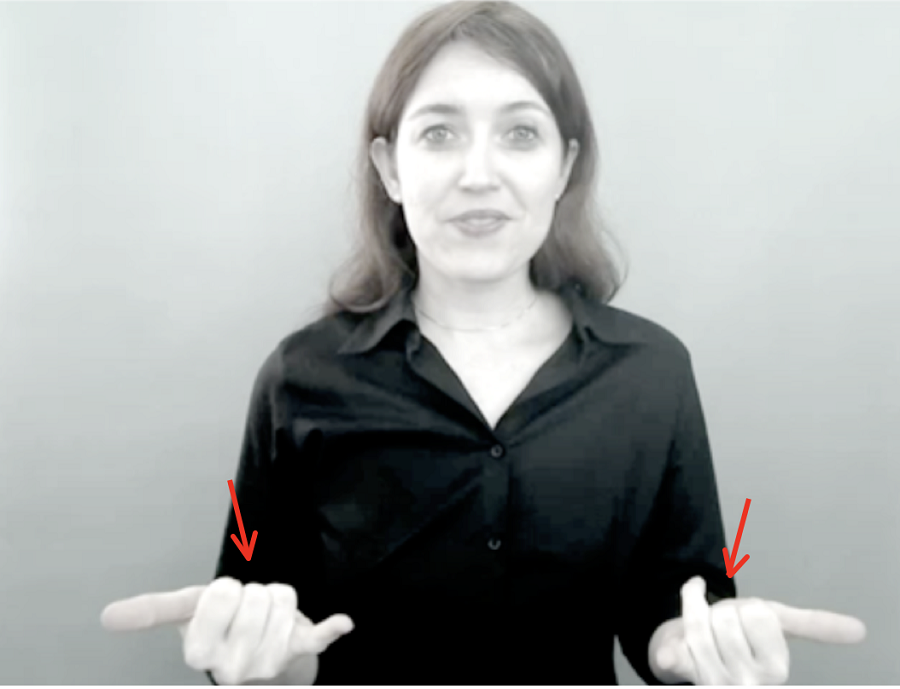
\includegraphics{../images/asl_now.png}
\caption{NOW}
\end{figure}

\newpage

{\large Question 3}\\

Source: Day 4 Discussion\\

Explain what we mean by saying that linguistic patterns are \underline{productive}.\\


\newpage

{\large Question 4}\\

Source: Homework 1, Question 3(b)\\

Explain why this is or is not a complete natural class in standard North American English.\\

{[f]}, {[θ]}, {[z]}, {[h]}


\newpage

{\large Question 5}\\

Source: Day 2 Handout, Part I, Question 11\\

How would this word be transcribed?\\ Follow-up question: Why did you use symbol [X] instead of symbol [Y]?\\

<little>


\newpage

\begin{center}
\textbf{{\color{red}{\HUGE END OF EXAM}}}\\

\end{center}
\newpage

\begin{center}
\textbf{{\color{blue}{\HUGE START OF EXAM\\}}}

\textbf{{\color{blue}{\HUGE Student ID: 7336\\}}}

\textbf{{\color{blue}{\HUGE 1:15 - 1:30 PM\\}}}

\end{center}
\newpage

{\large Question 1}\\

Source: Quiz 3, Question 2\\

L$_X$ has tri-syllabic roots. If L$_X$ does not allow non-identical high vowels to co-occur, which one of the following tri-syllabic vocalic sequences do you predict to be unattested in L$_X$? Explain why.\\

\begin{itemize} \item {[u...i...a]} \item {[a...i...a]} \item {[u...u...a]} \item {[a...i...i]} \end{itemize}


\newpage

{\large Question 2}\\

Source: Day 2 Discussion\\

Assuming a Standard North American English inventory, does this vowel need to have tenseness specified if you're giving a prose description? Why or why not?\\

{[u]}


\newpage

{\large Question 3}\\

Source: Day 7 Handout, Question 9\\

What is the basic analysis of vowel length in this dataset, and what are the key pieces of evidence?\\

\begin{figure}[H]
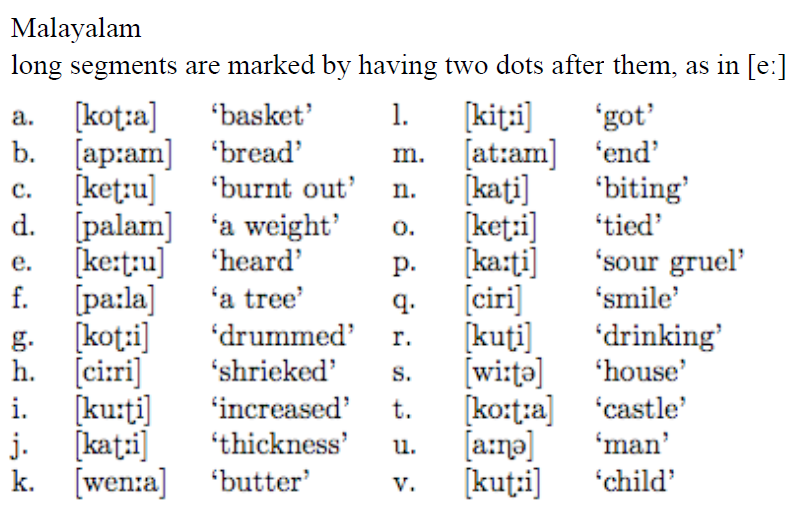
\includegraphics{../images/malayalam.png}
\end{figure}

\newpage

{\large Question 4}\\

Source: Quiz 1, Question 7\\

Is this sentence prescriptive or descriptive? Explain why.\\

In casual styles of speaking, English speakers frequently end sentences with prepositions, but ending sentences with prepositions is avoided in formal styles.


\newpage

{\large Question 5}\\

Source: Day 2 Handout\\

Is this a reasonable transcription of this word? Explain why.\\

<health>: {[hɛlð]}


\newpage

\begin{center}
\textbf{{\color{red}{\HUGE END OF EXAM}}}\\

\end{center}
\newpage

\begin{center}
\textbf{{\color{blue}{\HUGE START OF EXAM\\}}}

\textbf{{\color{blue}{\HUGE Student ID: 1715\\}}}

\textbf{{\color{blue}{\HUGE 1:30 - 1:45 PM\\}}}

\end{center}
\newpage

{\large Question 1}\\

Source: Day 5 Handout, Question 3\\

What evidence is there that there is a pattern in these data, assuming that these are the only CV and VC sequences that occur in some language?\\

{[sa]}, {[ʃi]}, {[za]}, {[ʒi]}, {[as]}, {[iʃ]}, {[az]}, {[iʒ]}


\newpage

{\large Question 2}\\

Source: Homework 1, Question 3(b)\\

Explain why this is or is not a complete natural class in standard North American English.\\

{[f]}, {[θ]}, {[z]}, {[h]}


\newpage

{\large Question 3}\\

Source: Day 2 Handout, Part II, Question 9\\

Explain how to figure out what the sound being produced is in this diagram.\\

\begin{figure}[H]
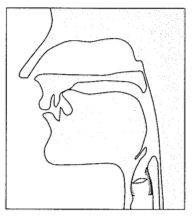
\includegraphics{../images/sagittal_t.png}
\end{figure}

\newpage

{\large Question 4}\\

Source: Day 6 Handout, Question 11\\

What do the two signs below tell you about the phonological status of \underline{handshape} in ASL, and why?\\

\begin{figure}[H]
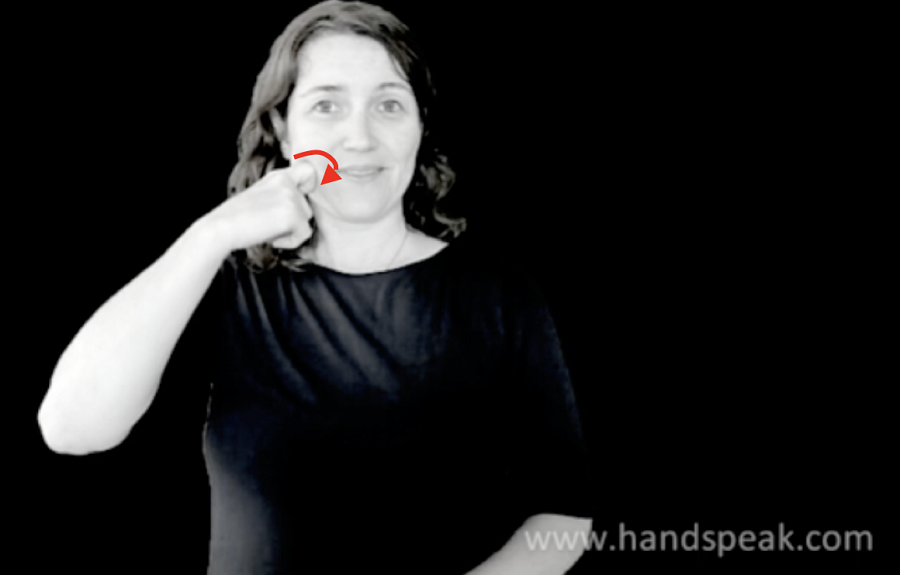
\includegraphics{../images/asl_apple.png}
\caption{APPLE}
\end{figure}
\begin{figure}[H]
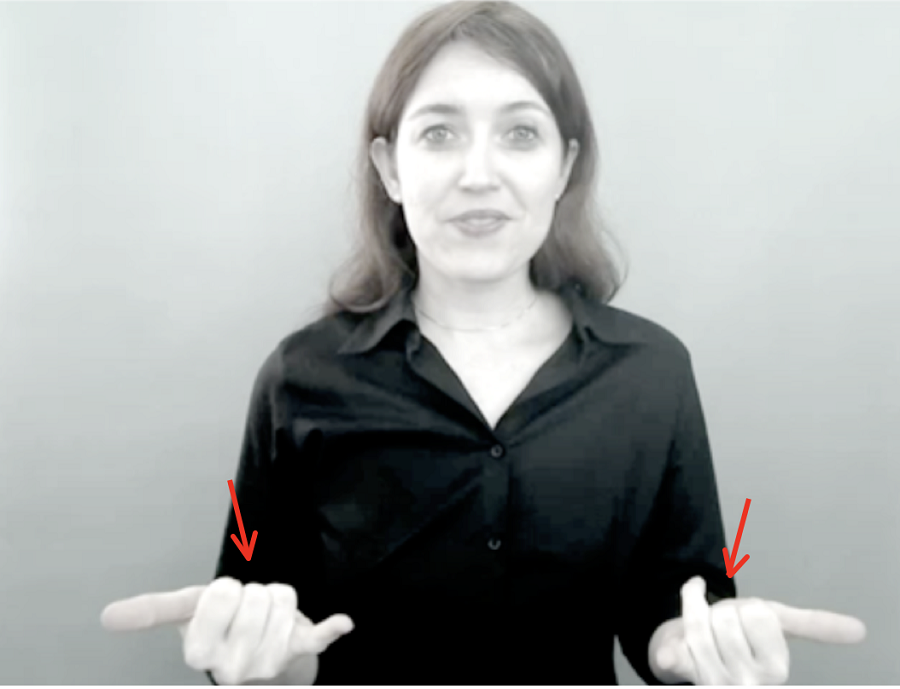
\includegraphics{../images/asl_now.png}
\caption{NOW}
\end{figure}

\newpage

{\large Question 5}\\

Source: Day 2 Handout, Part I, Question 11\\

How would this word be transcribed?\\ Follow-up question: Why did you use symbol [X] instead of symbol [Y]?\\

<cough>


\newpage

\begin{center}
\textbf{{\color{red}{\HUGE END OF EXAM}}}\\

\end{center}
\newpage

\begin{center}
\textbf{{\color{blue}{\HUGE START OF EXAM\\}}}

\textbf{{\color{blue}{\HUGE Student ID: 3288\\}}}

\textbf{{\color{blue}{\HUGE 1:45 - 2:00 PM\\}}}

\end{center}
\newpage

{\large Question 1}\\

Source: Quiz 3, Question 2\\

L$_X$ has tri-syllabic roots. If L$_X$ does not allow non-identical high vowels to co-occur, which one of the following tri-syllabic vocalic sequences do you predict to be unattested in L$_X$? Explain why.\\

\begin{itemize} \item {[u...i...a]} \item {[a...i...a]} \item {[u...u...a]} \item {[a...i...i]} \end{itemize}


\newpage

{\large Question 2}\\

Source: Day 2 Handout, Part II, Question 7\\

Is the symbol given a reasonable way to transcribe any of the sounds described below? If so, which one? If not, why not?\\

{[v]}

\begin{itemize} \item voiceless palatal affricate \item voiced velar nasal \item voiceless glottal fricative \item voiced labiodental fricative \item voiced interdental fricative \item voiced palatal fricative \end{itemize}


\newpage

{\large Question 3}\\

Source: Day 7 Handout, Question 9\\

What is the basic analysis of vowel length in this dataset, and what are the key pieces of evidence?\\

\begin{figure}[H]
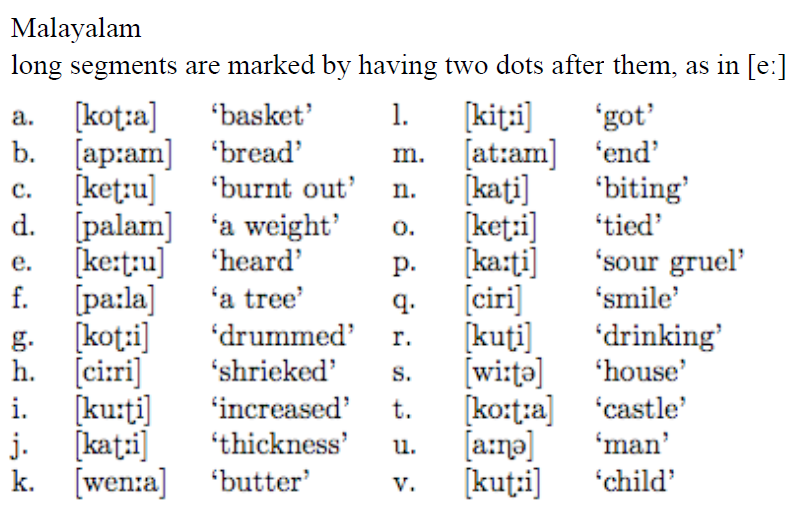
\includegraphics{../images/malayalam.png}
\end{figure}

\newpage

{\large Question 4}\\

Source: Day 2 Handout, Part I, Question 11\\

How would this word be transcribed?\\ Follow-up question: Why did you use symbol [X] instead of symbol [Y]?\\

<goat>


\newpage

{\large Question 5}\\

Source: Day 2 Handout, Part I, Question 11\\

How would this word be transcribed?\\ Follow-up question: Why did you use symbol [X] instead of symbol [Y]?\\

<finger>


\newpage

\begin{center}
\textbf{{\color{red}{\HUGE END OF EXAM}}}\\

\end{center}
\newpage

\begin{center}
\textbf{{\color{blue}{\HUGE START OF EXAM\\}}}

\textbf{{\color{blue}{\HUGE Student ID: 4656\\}}}

\textbf{{\color{blue}{\HUGE 2:00 - 2:15 PM\\}}}

\end{center}
\newpage

{\large Question 1}\\

Source: Quiz 3, Question 1\\

L$_X$ (Language X) has three vowels, [i], [a], and [u]. It has bi-syllabic roots like Kikuyu. It does not allow non-identical high vowels to co-occur. Of the following nine logically possible vocalic sequences, which ones should be unattested in L$_X$? Explain why.\\

\begin{itemize} \item {[i...i]} \item {[i...a]} \item {[i...u]} \item {[a...i]} \item {[a...a]} \item {[a...u]} \item {[u...i]} \item {[u...a]} \item {[u...u]} \end{itemize}


\newpage

{\large Question 2}\\

Source: Day 2 Handout, Part I, Question 11\\

How would this word be transcribed?\\ Follow-up question: Why did you use symbol [X] instead of symbol [Y]?\\

<cough>


\newpage

{\large Question 3}\\

Source: Day 2 Handout, Part II, Question 7\\

Is the symbol given a reasonable way to transcribe any of the sounds described below? If so, which one? If not, why not?\\

{[ʃ]}

\begin{itemize} \item voiceless palatal affricate \item voiced velar nasal \item voiceless glottal fricative \item voiced labiodental fricative \item voiced interdental fricative \item voiced palatal fricative \end{itemize}


\newpage

{\large Question 4}\\

Source: Day 2 Handout, Part II, Question 7\\

Is the symbol given a reasonable way to transcribe any of the sounds described below? If so, which one? If not, why not?\\

{[v]}

\begin{itemize} \item voiceless palatal affricate \item voiced velar nasal \item voiceless glottal fricative \item voiced labiodental fricative \item voiced interdental fricative \item voiced palatal fricative \end{itemize}


\newpage

{\large Question 5}\\

Source: Day 6 Handout, Question 11\\

What do the two signs below tell you about the phonological status of \underline{handshape} in ASL, and why?\\

\begin{figure}[H]
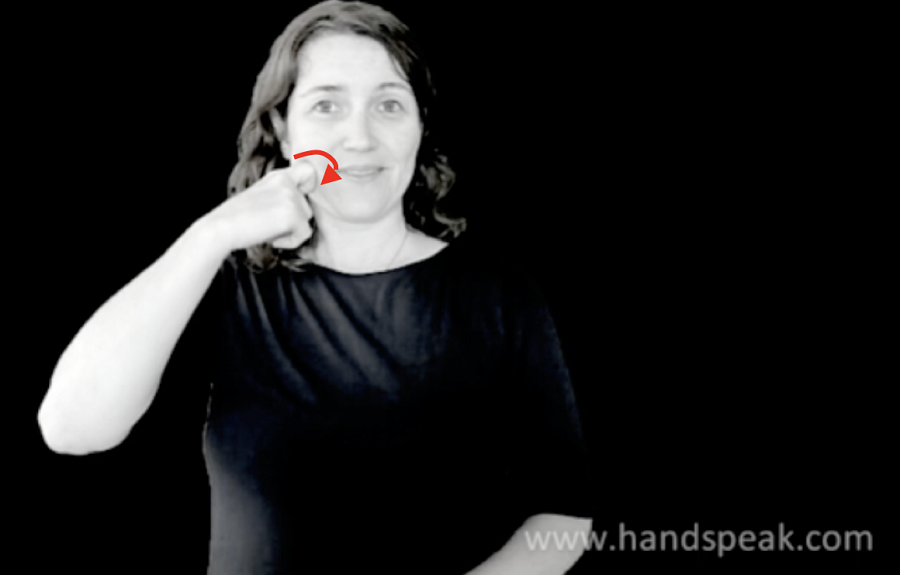
\includegraphics{../images/asl_apple.png}
\caption{APPLE}
\end{figure}
\begin{figure}[H]
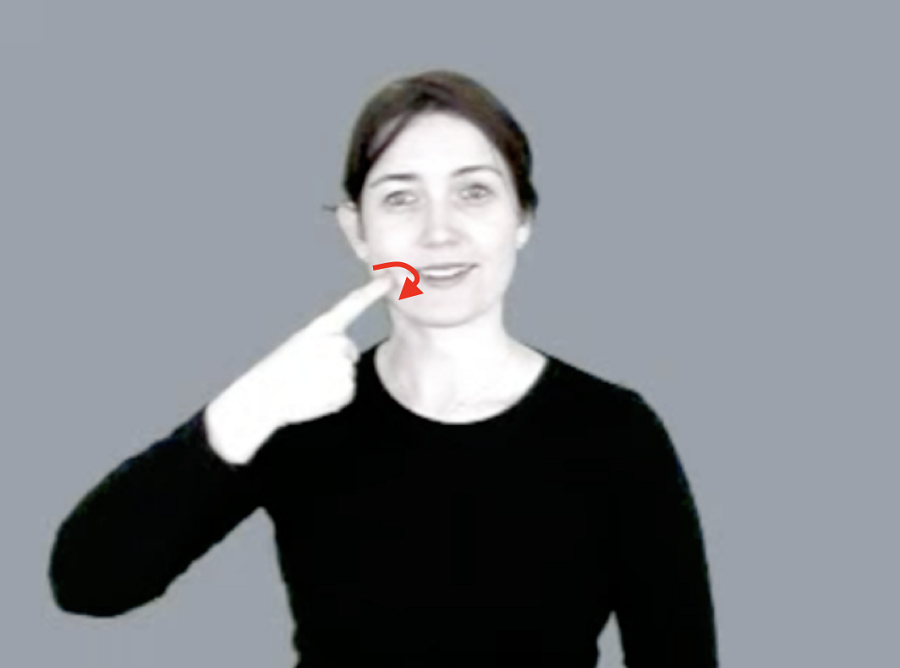
\includegraphics{../images/asl_candy.png}
\caption{CANDY}
\end{figure}

\newpage

\begin{center}
\textbf{{\color{red}{\HUGE END OF EXAM}}}\\

\end{center}
\newpage

\begin{center}
\textbf{{\color{blue}{\HUGE START OF EXAM\\}}}

\textbf{{\color{blue}{\HUGE Student ID: 3419\\}}}

\textbf{{\color{blue}{\HUGE 2:15 - 2:30 PM\\}}}

\end{center}
\newpage

{\large Question 1}\\

Source: Quiz 3, Question 2\\

L$_X$ has tri-syllabic roots. If L$_X$ does not allow non-identical high vowels to co-occur, which one of the following tri-syllabic vocalic sequences do you predict to be unattested in L$_X$? Explain why.\\

\begin{itemize} \item {[u...i...a]} \item {[a...i...a]} \item {[u...u...a]} \item {[a...i...i]} \end{itemize}


\newpage

{\large Question 2}\\

Source: Day 2 Handout, Part I, Question 11\\

How would this word be transcribed?\\ Follow-up question: Why did you use symbol [X] instead of symbol [Y]?\\

<vacuum>


\newpage

{\large Question 3}\\

Source: Day 7 Handout, Question 12\\

What is the basic analysis of oral and nasal vowels in this dataset, and what are the key pieces of evidence?\\

\begin{figure}[H]
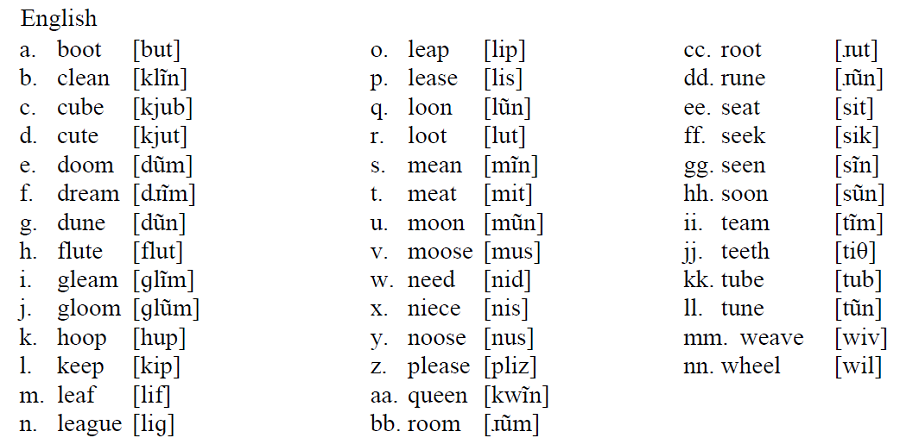
\includegraphics{../images/english12.png}
\end{figure}

\newpage

{\large Question 4}\\

Source: Day 6 Handout, Question 7\\

Explain how you would determine the phonological relationship between these two sounds (given below) in this dataset.\\

{[k]} and {[ɡ]}

\begin{figure}[H]
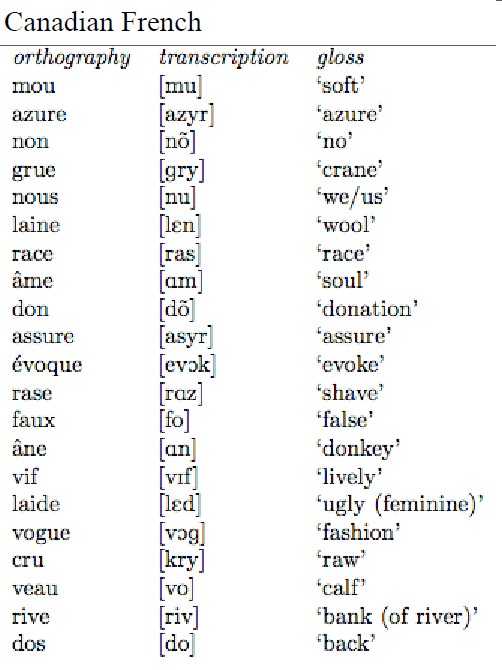
\includegraphics{../images/canadianfrench.png}
\end{figure}

\newpage

{\large Question 5}\\

Source: Day 2 Handout, Part II, Question 7\\

Is the symbol given a reasonable way to transcribe any of the sounds described below? If so, which one? If not, why not?\\

{[ʃ]}

\begin{itemize} \item voiceless palatal affricate \item voiced velar nasal \item voiceless glottal fricative \item voiced labiodental fricative \item voiced interdental fricative \item voiced palatal fricative \end{itemize}


\newpage

\begin{center}
\textbf{{\color{red}{\HUGE END OF EXAM}}}\\

\end{center}
\newpage

\begin{center}
\textbf{{\color{blue}{\HUGE START OF EXAM\\}}}

\textbf{{\color{blue}{\HUGE Student ID: 6801\\}}}

\textbf{{\color{blue}{\HUGE 2:30 - 2:45 PM\\}}}

\end{center}
\newpage

{\large Question 1}\\

Source: Day 5 Handout, Question 3\\

What evidence is there that there is a pattern in these data, assuming that these are the only CV and VC sequences that occur in some language?\\

{[sa]}, {[ʃi]}, {[za]}, {[ʒi]}, {[as]}, {[iʃ]}, {[az]}, {[iʒ]}


\newpage

{\large Question 2}\\

Source: Day 2 Discussion\\

Assuming a Standard North American English inventory, does this vowel need to have tenseness specified if you're giving a prose description? Why or why not?\\

{[ɛ]}


\newpage

{\large Question 3}\\

Source: Day 6 Handout, Question 11\\

What do the two signs below tell you about the phonological status of \underline{handshape} in ASL, and why?\\

\begin{figure}[H]
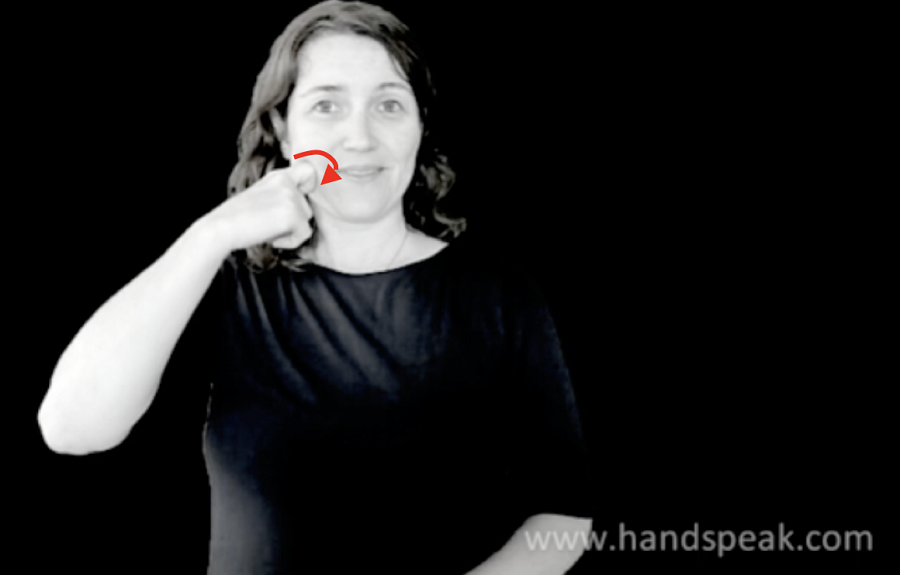
\includegraphics{../images/asl_apple.png}
\caption{APPLE}
\end{figure}
\begin{figure}[H]
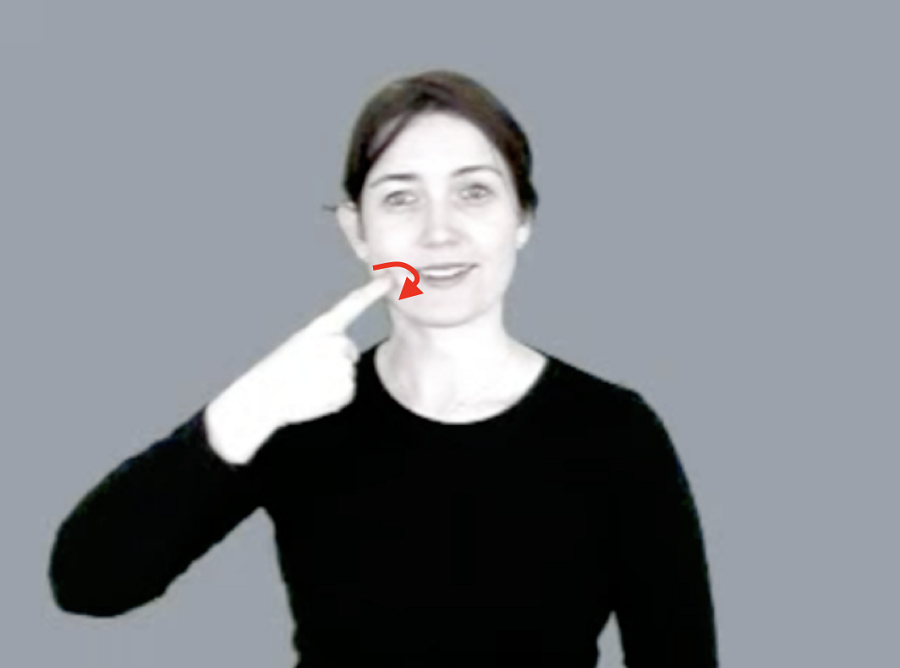
\includegraphics{../images/asl_candy.png}
\caption{CANDY}
\end{figure}

\newpage

{\large Question 4}\\

Source: Day 2 Handout, Part I, Question 11\\

How would this word be transcribed?\\ Follow-up question: Why did you use symbol [X] instead of symbol [Y]?\\

<little>


\newpage

{\large Question 5}\\

Source: Day 4 Handout, Question 2(iii)\\

Explain how you would figure out the meaning of this Swahili word.\\

{[watanipiɡa]}

\begin{figure}[H]
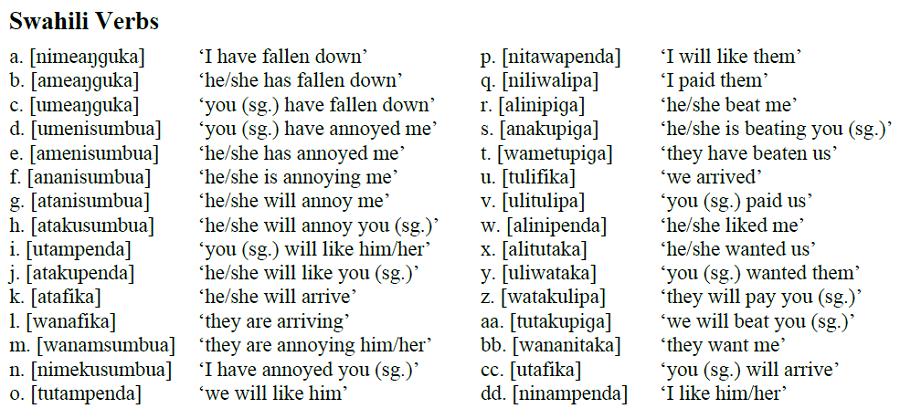
\includegraphics{../images/swahiliverbs.png}
\end{figure}

\newpage

\begin{center}
\textbf{{\color{red}{\HUGE END OF EXAM}}}\\

\end{center}
\newpage

\begin{center}
\textbf{{\color{blue}{\HUGE START OF EXAM\\}}}

\textbf{{\color{blue}{\HUGE Student ID: 5581\\}}}

\textbf{{\color{blue}{\HUGE 2:45 - 3:00 PM\\}}}

\end{center}
\newpage

{\large Question 1}\\

Source: Day 5 Handout, Question 5\\

How would you look for co-occurrence restrictions between [s] and the vowels that come after it in this dataset?\\

\begin{figure}[H]
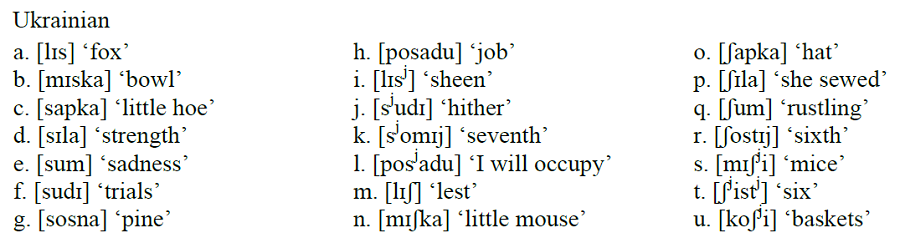
\includegraphics{../images/ukrainian.png}
\end{figure}

\newpage

{\large Question 2}\\

Source: Day 2 Handout, Part I, Question 11\\

How would this word be transcribed?\\ Follow-up question: Why did you use symbol [X] instead of symbol [Y]?\\

<cough>


\newpage

{\large Question 3}\\

Source: Day 6 Handout, Question 11\\

What do the two signs below tell you about the phonological status of \underline{handshape} in ASL, and why?\\

\begin{figure}[H]
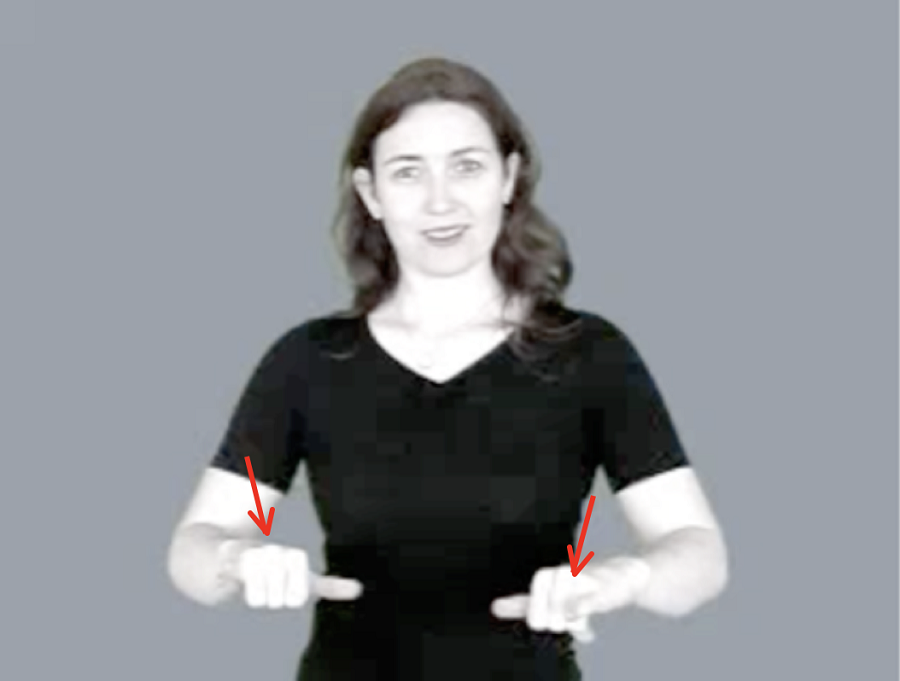
\includegraphics{../images/asl_stay.png}
\caption{STAY}
\end{figure}
\begin{figure}[H]
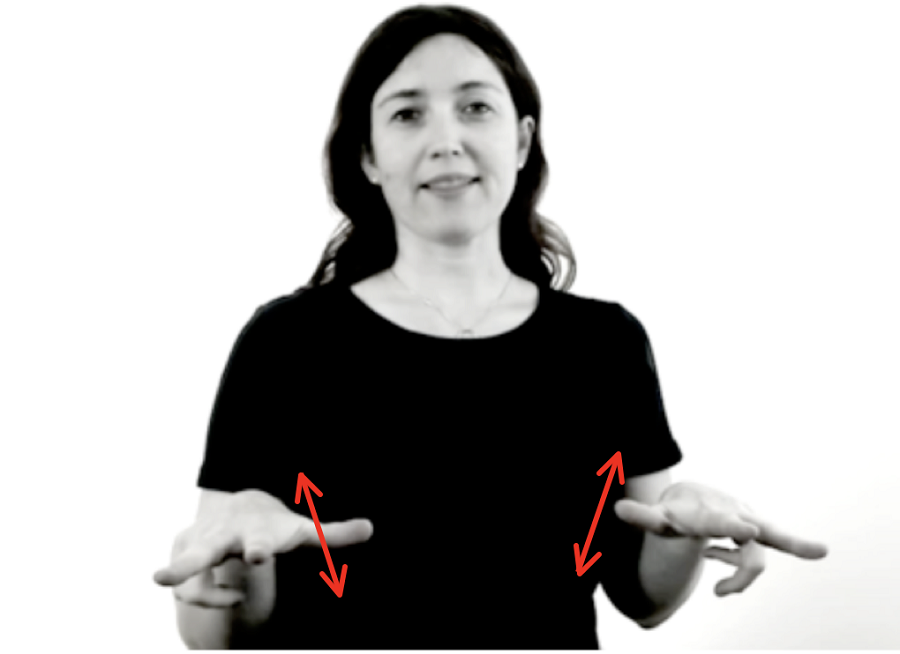
\includegraphics{../images/asl_awkward.png}
\caption{AWKWARD}
\end{figure}

\newpage

{\large Question 4}\\

Source: Day 7 Handout, Question 2\\

Explain whether the rule below would apply to the form shown, and if so, what the effect of the rule would be. Assume the vowel inventory [i], [ɪ], [e], [ɛ], [ɑ], [u], [ʊ], [o], [ɔ].\\

/emɛs/

{[high vowel]} →  {[unround, front]} / {[front vowel]} C$_0$ \_\_ 


\newpage

{\large Question 5}\\

Source: Day 2 Handout, Part II, Question 7\\

Is the symbol given a reasonable way to transcribe any of the sounds described below? If so, which one? If not, why not?\\

{[n]}

\begin{itemize} \item voiceless palatal affricate \item voiced velar nasal \item voiceless glottal fricative \item voiced labiodental fricative \item voiced interdental fricative \item voiced palatal fricative \end{itemize}


\newpage

\begin{center}
\textbf{{\color{red}{\HUGE END OF EXAM}}}\\

\end{center}
\newpage

\begin{center}
\textbf{{\color{blue}{\HUGE START OF EXAM\\}}}

\textbf{{\color{blue}{\HUGE Student ID: 3420\\}}}

\textbf{{\color{blue}{\HUGE 3:00 - 3:15 PM\\}}}

\end{center}
\newpage

{\large Question 1}\\

Source: Day 5 Handout, Question 5\\

How would you look for co-occurrence restrictions between [s] and the vowels that come after it in this dataset?\\

\begin{figure}[H]
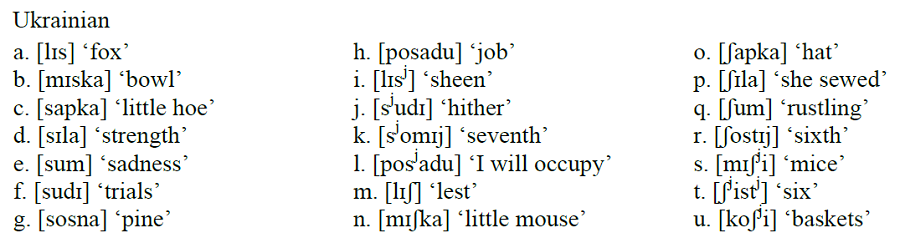
\includegraphics{../images/ukrainian.png}
\end{figure}

\newpage

{\large Question 2}\\

Source: Day 2 Handout, Part II, Question 7\\

Is the symbol given a reasonable way to transcribe any of the sounds described below? If so, which one? If not, why not?\\

{[t͡ʃ]}

\begin{itemize} \item voiceless palatal affricate \item voiced velar nasal \item voiceless glottal fricative \item voiced labiodental fricative \item voiced interdental fricative \item voiced palatal fricative \end{itemize}


\newpage

{\large Question 3}\\

Source: Day 2 Handout\\

Is this a reasonable transcription of this word? Explain why.\\

<philosophy>: {[fəlɑsəfi]}


\newpage

{\large Question 4}\\

Source: Day 6 Handout, Question 11\\

What do the two signs below tell you about the phonological status of \underline{handshape} in ASL, and why?\\

\begin{figure}[H]
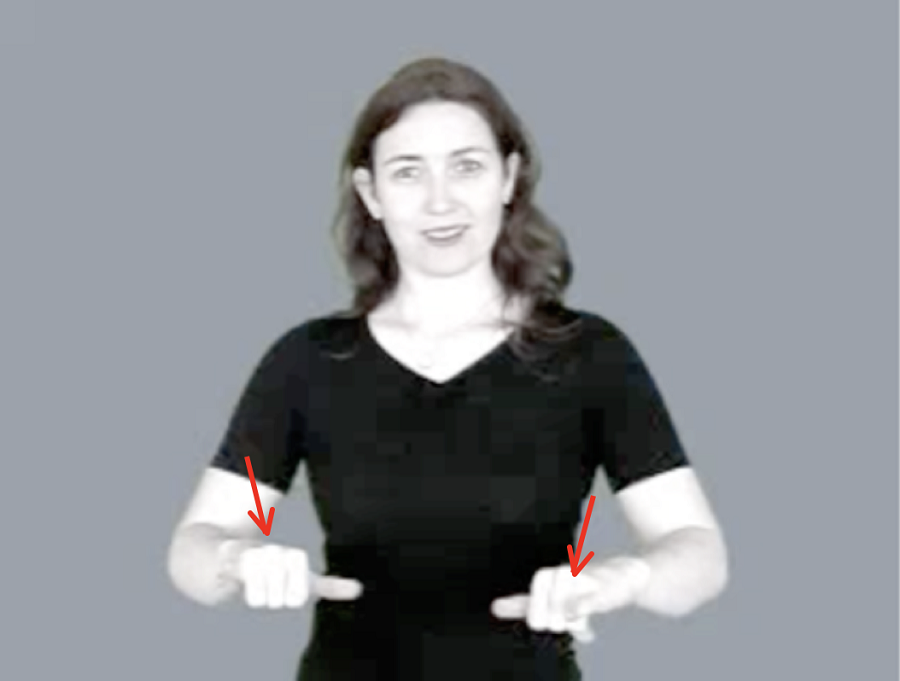
\includegraphics{../images/asl_stay.png}
\caption{STAY}
\end{figure}
\begin{figure}[H]
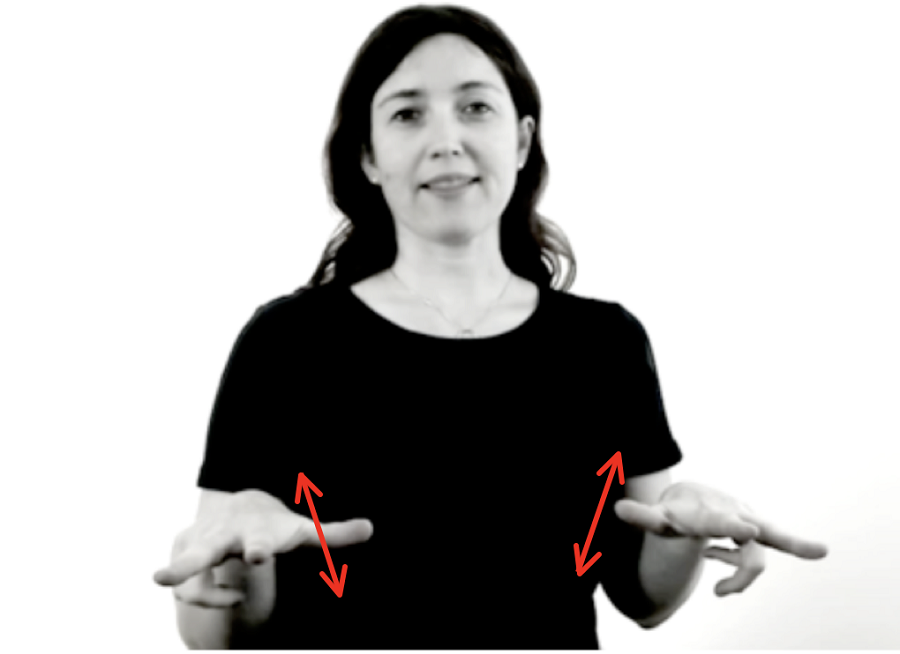
\includegraphics{../images/asl_awkward.png}
\caption{AWKWARD}
\end{figure}

\newpage

{\large Question 5}\\

Source: Day 2 Handout, Part I, Question 3\\

Explain why people might legitimately disagree about how many sounds this particular word contains.\\

<rice>


\newpage

\begin{center}
\textbf{{\color{red}{\HUGE END OF EXAM}}}\\

\end{center}
\newpage

\begin{center}
\textbf{{\color{blue}{\HUGE START OF EXAM\\}}}

\textbf{{\color{blue}{\HUGE Student ID: 6427\\}}}

\textbf{{\color{blue}{\HUGE 3:15 - 3:30 PM\\}}}

\end{center}
\newpage

{\large Question 1}\\

Source: Day 5 Handout, Question 3\\

What evidence is there that there is a pattern in these data, assuming that these are the only CV and VC sequences that occur in some language?\\

{[sa]}, {[ʃi]}, {[za]}, {[ʒi]}, {[as]}, {[iʃ]}, {[az]}, {[iʒ]}


\newpage

{\large Question 2}\\

Source: Day 2 Handout, Part I, Question 11\\

How would this word be transcribed?\\ Follow-up question: Why did you use symbol [X] instead of symbol [Y]?\\

<bird>


\newpage

{\large Question 3}\\

Source: Day 2 Handout, Part I, Question 11\\

How would this word be transcribed?\\ Follow-up question: Why did you use symbol [X] instead of symbol [Y]?\\

<wealth>


\newpage

{\large Question 4}\\

Source: Day 2 Handout, Part II, Question 7\\

Is the symbol given a reasonable way to transcribe any of the sounds described below? If so, which one? If not, why not?\\

{[v]}

\begin{itemize} \item voiceless palatal affricate \item voiced velar nasal \item voiceless glottal fricative \item voiced labiodental fricative \item voiced interdental fricative \item voiced palatal fricative \end{itemize}


\newpage

{\large Question 5}\\

Source: Day 6 Handout, Question 11\\

What do the two signs below tell you about the phonological status of \underline{handshape} in ASL, and why?\\

\begin{figure}[H]
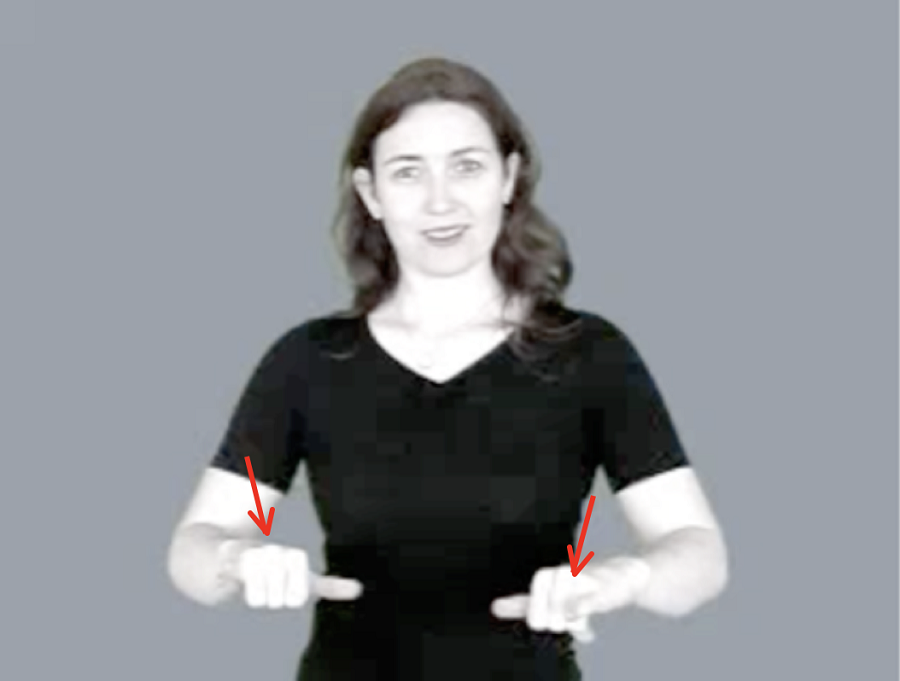
\includegraphics{../images/asl_stay.png}
\caption{STAY}
\end{figure}
\begin{figure}[H]
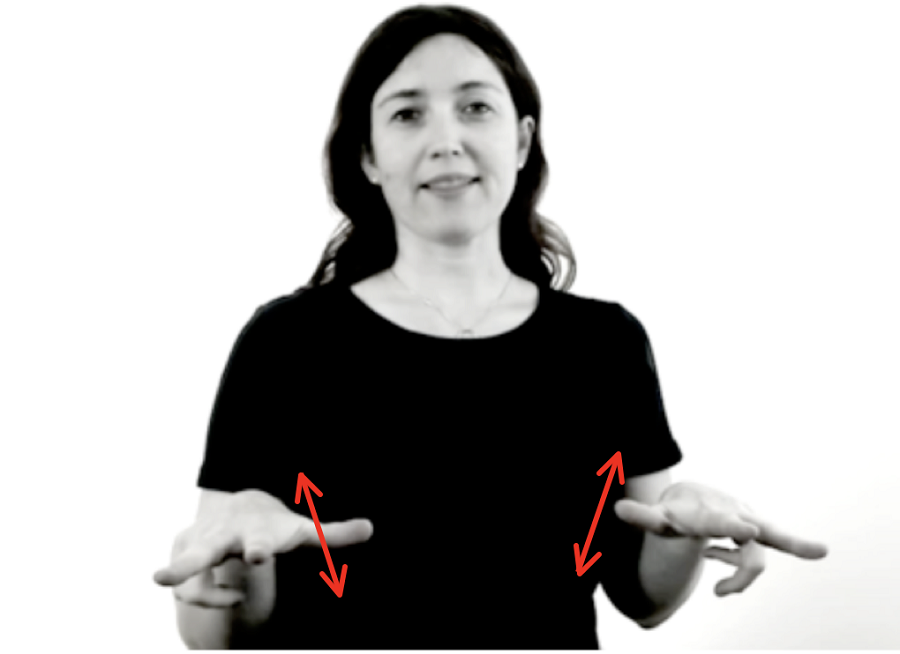
\includegraphics{../images/asl_awkward.png}
\caption{AWKWARD}
\end{figure}

\newpage

\begin{center}
\textbf{{\color{red}{\HUGE END OF EXAM}}}\\

\end{center}
\newpage

\begin{center}
\textbf{{\color{blue}{\HUGE START OF EXAM\\}}}

\textbf{{\color{blue}{\HUGE Student ID: 1956\\}}}

\textbf{{\color{blue}{\HUGE 3:30 - 3:45 PM\\}}}

\end{center}
\newpage

{\large Question 1}\\

Source: Day 5 Handout, Question 5\\

How would you look for co-occurrence restrictions between [s] and the vowels that come after it in this dataset?\\

\begin{figure}[H]
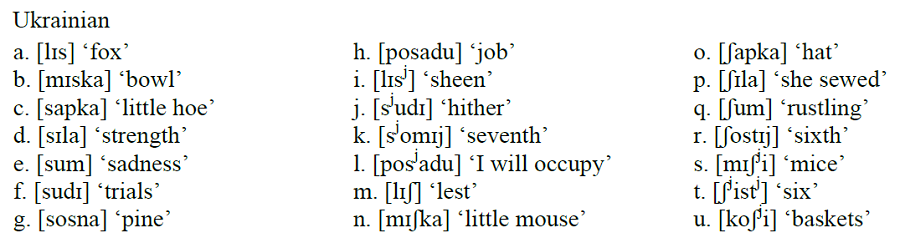
\includegraphics{../images/ukrainian.png}
\end{figure}

\newpage

{\large Question 2}\\

Source: Day 2 Discussion\\

Assuming a Standard North American English inventory, does this vowel need to have tenseness specified if you're giving a prose description? Why or why not?\\

{[ɔ]}


\newpage

{\large Question 3}\\

Source: Day 2 Handout, Part I, Question 11\\

How would this word be transcribed?\\ Follow-up question: Why did you use symbol [X] instead of symbol [Y]?\\

<wealth>


\newpage

{\large Question 4}\\

Source: Day 7 Handout, Question 12\\

What is the basic analysis of oral and nasal vowels in this dataset, and what are the key pieces of evidence?\\

\begin{figure}[H]
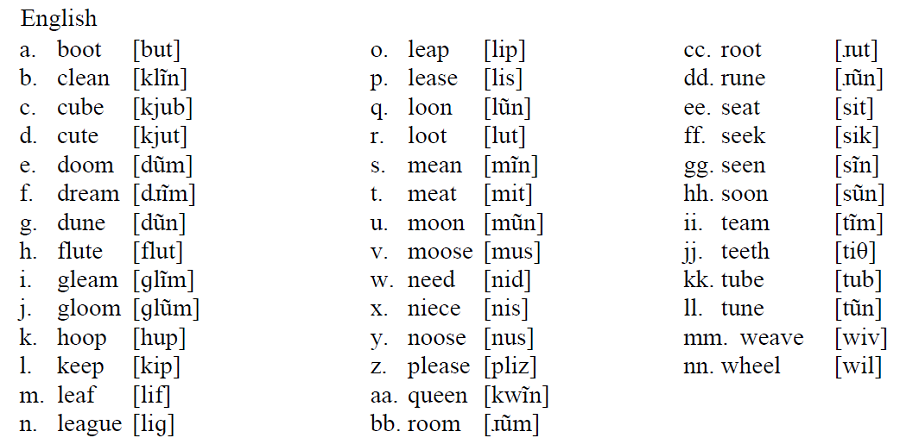
\includegraphics{../images/english12.png}
\end{figure}

\newpage

{\large Question 5}\\

Source: Day 2 Discussion\\

Assuming a Standard North American English inventory, does this vowel need to have tenseness specified if you're giving a prose description? Why or why not?\\

{[i]}


\newpage

\begin{center}
\textbf{{\color{red}{\HUGE END OF EXAM}}}\\

\end{center}
\newpage

\begin{center}
\textbf{{\color{blue}{\HUGE START OF EXAM\\}}}

\textbf{{\color{blue}{\HUGE Student ID: 5540\\}}}

\textbf{{\color{blue}{\HUGE 3:45 - 4:00 PM\\}}}

\end{center}
\newpage

{\large Question 1}\\

Source: Day 5 Handout, Question 5\\

How would you look for co-occurrence restrictions between [s] and the vowels that come after it in this dataset?\\

\begin{figure}[H]
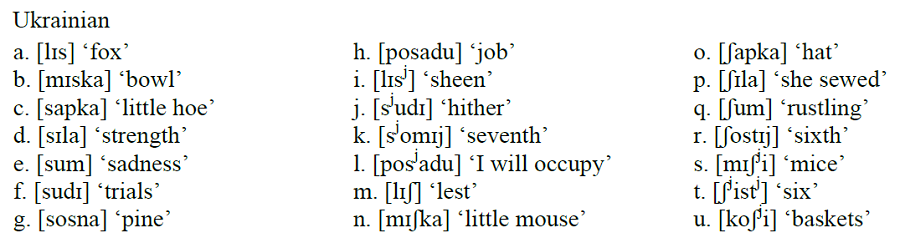
\includegraphics{../images/ukrainian.png}
\end{figure}

\newpage

{\large Question 2}\\

Source: Day 2 Handout, Part I, Question 11\\

How would this word be transcribed?\\ Follow-up question: Why did you use symbol [X] instead of symbol [Y]?\\

<bird>


\newpage

{\large Question 3}\\

Source: Quiz 4, Question 5\\

What phonological relationships does this example show among the sounds [m], [n], and [ŋ], and why?\\

\begin{figure}[H]
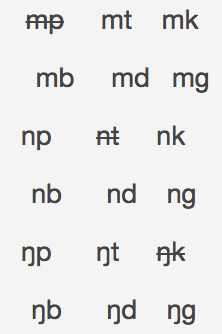
\includegraphics{../images/quiz4question5_d.png}
\end{figure}

\newpage

{\large Question 4}\\

Source: Day 2 Handout, Part II, Question 9\\

Explain how to figure out what the sound being produced is in this diagram.\\

\begin{figure}[H]
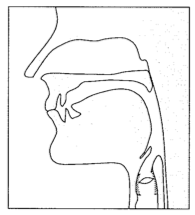
\includegraphics{../images/sagittal_p.png}
\end{figure}

\newpage

{\large Question 5}\\

Source: Day 6 Handout, Question 11\\

What do the two signs below tell you about the phonological status of \underline{handshape} in ASL, and why?\\

\begin{figure}[H]
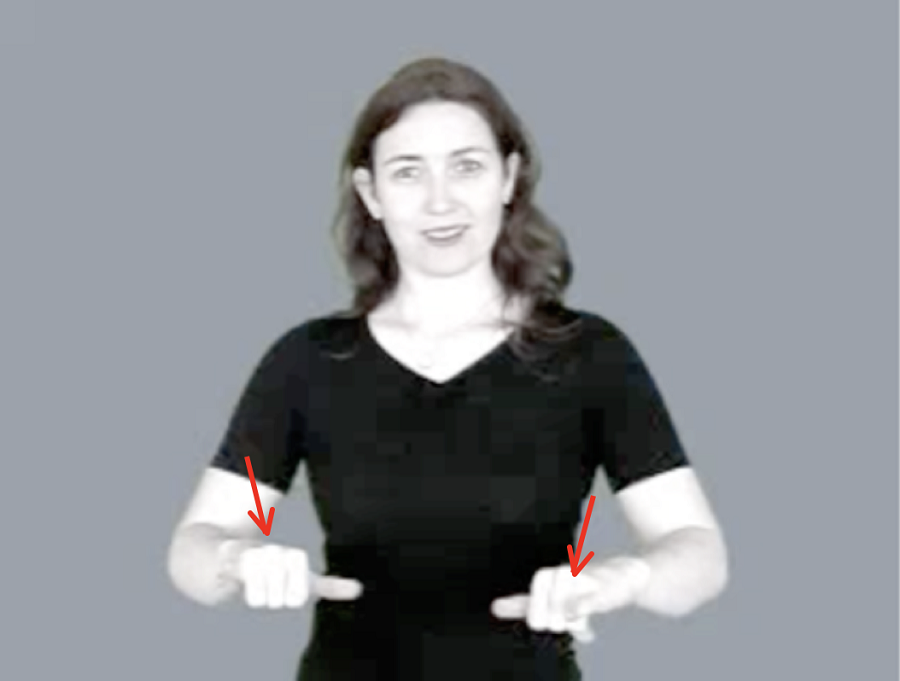
\includegraphics{../images/asl_stay.png}
\caption{STAY}
\end{figure}
\begin{figure}[H]
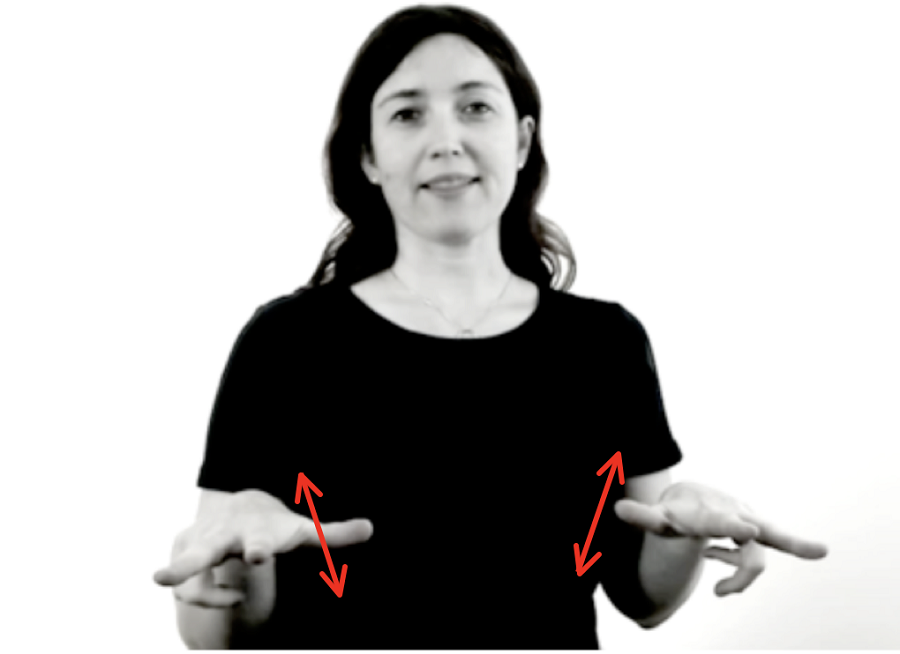
\includegraphics{../images/asl_awkward.png}
\caption{AWKWARD}
\end{figure}

\newpage

\begin{center}
\textbf{{\color{red}{\HUGE END OF EXAM}}}\\

\end{center}
\newpage

\begin{center}
\textbf{{\color{blue}{\HUGE START OF EXAM\\}}}

\textbf{{\color{blue}{\HUGE Student ID: 4066\\}}}

\textbf{{\color{blue}{\HUGE 4:00 - 4:15 PM\\}}}

\end{center}
\newpage

{\large Question 1}\\

Source: Quiz 3, Question 1\\

L$_X$ (Language X) has three vowels, [i], [a], and [u]. It has bi-syllabic roots like Kikuyu. It does not allow non-identical high vowels to co-occur. Of the following nine logically possible vocalic sequences, which ones should be unattested in L$_X$? Explain why.\\

\begin{itemize} \item {[i...i]} \item {[i...a]} \item {[i...u]} \item {[a...i]} \item {[a...a]} \item {[a...u]} \item {[u...i]} \item {[u...a]} \item {[u...u]} \end{itemize}


\newpage

{\large Question 2}\\

Source: Quiz 2, Question 11\\

Does the morpheme ‘eye’ occur in this word? Why or why not?\\

<eyeglasses>


\newpage

{\large Question 3}\\

Source: Day 2 Handout, Part I, Question 11\\

How would this word be transcribed?\\ Follow-up question: Why did you use symbol [X] instead of symbol [Y]?\\

<finger>


\newpage

{\large Question 4}\\

Source: Homework 1, Question 3(a)\\

Could this image be the result of producing the sound represented by the given IPA symbol? Why or why not?\\

{[d]}

\begin{figure}[H]
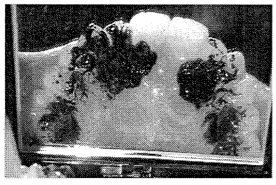
\includegraphics{../images/staticpalatography_fricative.png}
\end{figure}

\newpage

{\large Question 5}\\

Source: Day 6 Handout, Question 11\\

What do the two signs below tell you about the phonological status of \underline{handshape} in ASL, and why?\\

\begin{figure}[H]
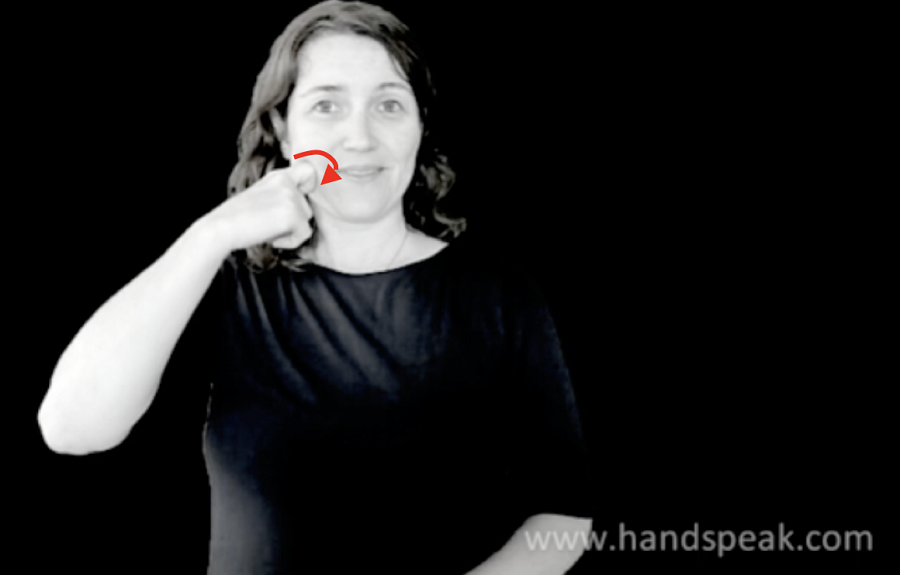
\includegraphics{../images/asl_apple.png}
\caption{APPLE}
\end{figure}
\begin{figure}[H]
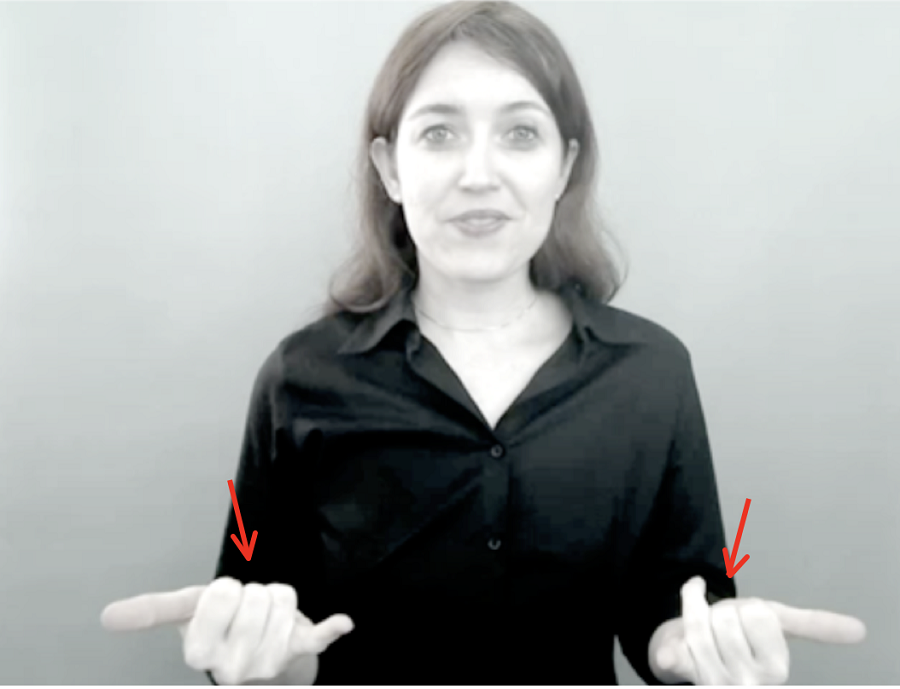
\includegraphics{../images/asl_now.png}
\caption{NOW}
\end{figure}

\newpage

\begin{center}
\textbf{{\color{red}{\HUGE END OF EXAM}}}\\

\end{center}
\newpage

\begin{center}
\textbf{{\color{blue}{\HUGE START OF EXAM\\}}}

\textbf{{\color{blue}{\HUGE Student ID: 9450\\}}}

\textbf{{\color{blue}{\HUGE 4:15 - 4:30 PM\\}}}

\end{center}
\newpage

{\large Question 1}\\

Source: Quiz 3, Question 1\\

L$_X$ (Language X) has three vowels, [i], [a], and [u]. It has bi-syllabic roots like Kikuyu. It does not allow non-identical high vowels to co-occur. Of the following nine logically possible vocalic sequences, which ones should be unattested in L$_X$? Explain why.\\

\begin{itemize} \item {[i...i]} \item {[i...a]} \item {[i...u]} \item {[a...i]} \item {[a...a]} \item {[a...u]} \item {[u...i]} \item {[u...a]} \item {[u...u]} \end{itemize}


\newpage

{\large Question 2}\\

Source: Day 2 Handout, Part II, Question 7\\

Is the symbol given a reasonable way to transcribe any of the sounds described below? If so, which one? If not, why not?\\

{[t͡ʃ]}

\begin{itemize} \item voiceless palatal affricate \item voiced velar nasal \item voiceless glottal fricative \item voiced labiodental fricative \item voiced interdental fricative \item voiced palatal fricative \end{itemize}


\newpage

{\large Question 3}\\

Source: Homework 1, Question 3(b)\\

Explain why this is or is not a complete natural class in standard North American English.\\

{[ɔ]}, {[ʊ]}, {[u]}, {[oʊ]}


\newpage

{\large Question 4}\\

Source: Day 2 Handout, Part I, Question 11\\

How would this word be transcribed?\\ Follow-up question: Why did you use symbol [X] instead of symbol [Y]?\\

<frog>


\newpage

{\large Question 5}\\

Source: Day 6 Handout, Question 11\\

What do the two signs below tell you about the phonological status of \underline{handshape} in ASL, and why?\\

\begin{figure}[H]
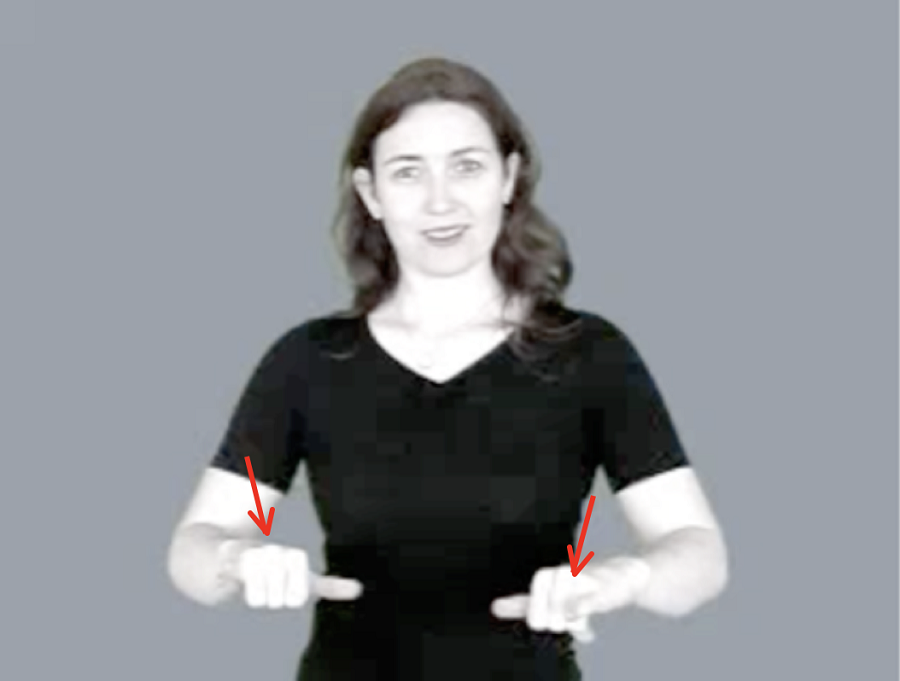
\includegraphics{../images/asl_stay.png}
\caption{STAY}
\end{figure}
\begin{figure}[H]
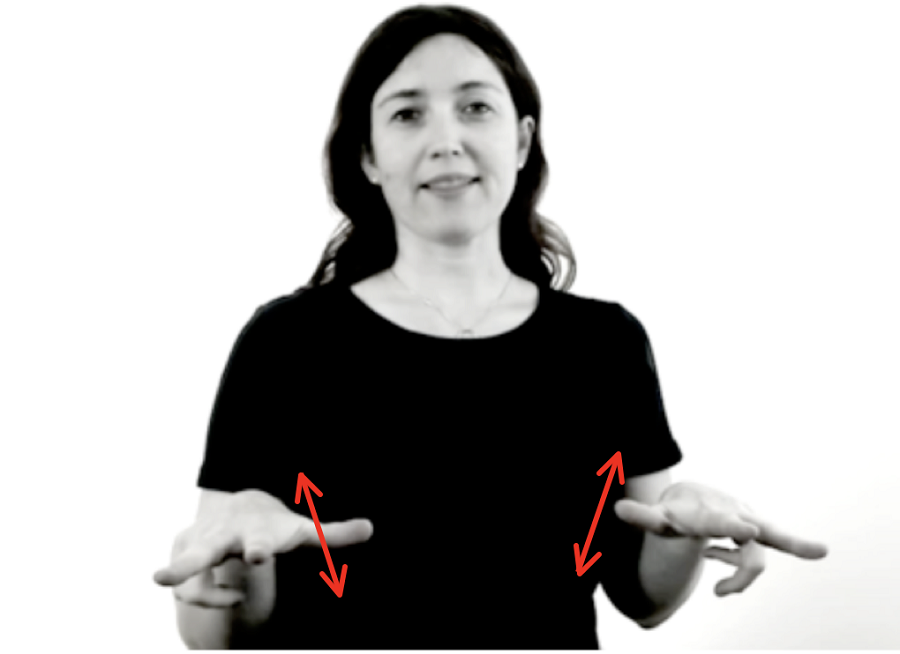
\includegraphics{../images/asl_awkward.png}
\caption{AWKWARD}
\end{figure}

\newpage

\begin{center}
\textbf{{\color{red}{\HUGE END OF EXAM}}}\\

\end{center}
\newpage

\begin{center}
\textbf{{\color{blue}{\HUGE START OF EXAM\\}}}

\textbf{{\color{blue}{\HUGE Student ID: 9918\\}}}

\textbf{{\color{blue}{\HUGE 4:30 - 4:45 PM\\}}}

\end{center}
\newpage

{\large Question 1}\\

Source: Quiz 3, Question 2\\

L$_X$ has tri-syllabic roots. If L$_X$ does not allow non-identical high vowels to co-occur, which one of the following tri-syllabic vocalic sequences do you predict to be unattested in L$_X$? Explain why.\\

\begin{itemize} \item {[u...i...a]} \item {[a...i...a]} \item {[u...u...a]} \item {[a...i...i]} \end{itemize}


\newpage

{\large Question 2}\\

Source: Homework 1, Question 3(b)\\

Explain why this is or is not a complete natural class in standard North American English.\\

{[ɑ]}, {[u]}


\newpage

{\large Question 3}\\

Source: Day 2 Handout, Part I, Question 11\\

How would this word be transcribed?\\ Follow-up question: Why did you use symbol [X] instead of symbol [Y]?\\

<frog>


\newpage

{\large Question 4}\\

Source: Day 7 Handout, Question 9\\

What is the basic analysis of vowel length in this dataset, and what are the key pieces of evidence?\\

\begin{figure}[H]
\includegraphics{../images/malayalam.png}
\end{figure}

\newpage

{\large Question 5}\\

Source: Day 2 Handout, Part II, Question 7\\

Is the symbol given a reasonable way to transcribe any of the sounds described below? If so, which one? If not, why not?\\

{[ʃ]}

\begin{itemize} \item voiceless palatal affricate \item voiced velar nasal \item voiceless glottal fricative \item voiced labiodental fricative \item voiced interdental fricative \item voiced palatal fricative \end{itemize}


\newpage

\begin{center}
\textbf{{\color{red}{\HUGE END OF EXAM}}}\\

\end{center}
\newpage

\begin{center}
\textbf{{\color{blue}{\HUGE START OF EXAM\\}}}

\textbf{{\color{blue}{\HUGE Student ID: 6948\\}}}

\textbf{{\color{blue}{\HUGE 4:45 - 5:00 PM\\}}}

\end{center}
\newpage

{\large Question 1}\\

Source: Quiz 3, Question 2\\

L$_X$ has tri-syllabic roots. If L$_X$ does not allow non-identical high vowels to co-occur, which one of the following tri-syllabic vocalic sequences do you predict to be unattested in L$_X$? Explain why.\\

\begin{itemize} \item {[u...i...a]} \item {[a...i...a]} \item {[u...u...a]} \item {[a...i...i]} \end{itemize}


\newpage

{\large Question 2}\\

Source: Day 2 Handout, Part I, Question 11\\

How would this word be transcribed?\\ Follow-up question: Why did you use symbol [X] instead of symbol [Y]?\\

<finger>


\newpage

{\large Question 3}\\

Source: Day 2 Handout, Part I, Question 11\\

How would this word be transcribed?\\ Follow-up question: Why did you use symbol [X] instead of symbol [Y]?\\

<frog>


\newpage

{\large Question 4}\\

Source: Day 6 Handout, Question 11\\

What do the two signs below tell you about the phonological status of \underline{handshape} in ASL, and why?\\

\begin{figure}[H]
\includegraphics{../images/asl_apple.png}
\caption{APPLE}
\end{figure}
\begin{figure}[H]
\includegraphics{../images/asl_now.png}
\caption{NOW}
\end{figure}

\newpage

{\large Question 5}\\

Source: Homework 1, Question 3(b)\\

Explain why this is or is not a complete natural class in standard North American English.\\

{[ɔ]}, {[ʊ]}, {[u]}, {[oʊ]}


\newpage

\begin{center}
\textbf{{\color{red}{\HUGE END OF EXAM}}}\\

\end{center}
\newpage

\begin{center}
\textbf{{\color{blue}{\HUGE START OF EXAM\\}}}

\textbf{{\color{blue}{\HUGE Student ID: 3347\\}}}

\textbf{{\color{blue}{\HUGE 5:00 - 5:15 PM\\}}}

\end{center}
\newpage

{\large Question 1}\\

Source: Day 5 Handout, Question 5\\

How would you look for co-occurrence restrictions between [s] and the vowels that come after it in this dataset?\\

\begin{figure}[H]
\includegraphics{../images/ukrainian.png}
\end{figure}

\newpage

{\large Question 2}\\

Source: Homework 2, Question 1\\

What would this Klingon phrase below be in English? How do you know?\\

{[pɑqqʰoqʰvetɬvo]}

\begin{figure}[H]
\includegraphics{../images/klingon.png}
\end{figure}

\newpage

{\large Question 3}\\

Source: Day 6 Handout, Question 11\\

What do the two signs below tell you about the phonological status of \underline{handshape} in ASL, and why?\\

\begin{figure}[H]
\includegraphics{../images/asl_apple.png}
\caption{APPLE}
\end{figure}
\begin{figure}[H]
\includegraphics{../images/asl_candy.png}
\caption{CANDY}
\end{figure}

\newpage

{\large Question 4}\\

Source: Day 2 Handout, Part I, Question 11\\

How would this word be transcribed?\\ Follow-up question: Why did you use symbol [X] instead of symbol [Y]?\\

<finger>


\newpage

{\large Question 5}\\

Source: Homework 1, Question 3(b)\\

Explain why this is or is not a complete natural class in standard North American English.\\

{[ɑ]}, {[u]}


\newpage

\begin{center}
\textbf{{\color{red}{\HUGE END OF EXAM}}}\\

\end{center}
\newpage

\begin{center}
\textbf{{\color{blue}{\HUGE START OF EXAM\\}}}

\textbf{{\color{blue}{\HUGE Student ID: 1887\\}}}

\textbf{{\color{blue}{\HUGE 5:15 - 5:30 PM\\}}}

\end{center}
\newpage

{\large Question 1}\\

Source: Quiz 3, Question 2\\

L$_X$ has tri-syllabic roots. If L$_X$ does not allow non-identical high vowels to co-occur, which one of the following tri-syllabic vocalic sequences do you predict to be unattested in L$_X$? Explain why.\\

\begin{itemize} \item {[u...i...a]} \item {[a...i...a]} \item {[u...u...a]} \item {[a...i...i]} \end{itemize}


\newpage

{\large Question 2}\\

Source: Day 2 Handout, Part II, Question 13\\

Explain why this image does or does not match the description.\\

\begin{itemize} \item A one-handed sign. \item Location: In front of signer’s chin. \item Handshape: Starts with an “L” shape; proximal joint of index finger folds down during the sign. \item Movement: Hand starts on far side of signer’s body and moves horizontally straight across. \end{itemize}

\begin{figure}[H]
\includegraphics{../images/taiwansign_jealous.png}
\caption{JEALOUS}
\end{figure}

\newpage

{\large Question 3}\\

Source: Day 7 Handout, Question 9\\

What is the basic analysis of vowel length in this dataset, and what are the key pieces of evidence?\\

\begin{figure}[H]
\includegraphics{../images/malayalam.png}
\end{figure}

\newpage

{\large Question 4}\\

Source: Day 2 Handout, Part I, Question 11\\

How would this word be transcribed?\\ Follow-up question: Why did you use symbol [X] instead of symbol [Y]?\\

<frog>


\newpage

{\large Question 5}\\

Source: Day 2 Handout, Part I, Question 11\\

How would this word be transcribed?\\ Follow-up question: Why did you use symbol [X] instead of symbol [Y]?\\

<little>


\newpage

\begin{center}
\textbf{{\color{red}{\HUGE END OF EXAM}}}\\

\end{center}
\newpage

\end{document}

